\chapter{Experiments and Results}
\label{chp:b6}

We conducted various experiments for different scenarios in the simulation and
real miniature courses. In this chapter, we introduce our courses and datasets
collected from the courses. We evaluate our semantic segmentation and
classification deep learning models based on these datasets. We then demostrate
the behavior of our car on different traffic scenarios.

\section{Race Courses and Datasets}

Our experiments are based on four different courses. The first course is the
course provided by OpenZeka  two days before the competition, so it was not
available to us during the development. The second course is the one we
constructed in our laboratory, which is spatially no larger than the bridge
area of the actual competition course. We used it to collect simple images and
test our hardware setup to ensure the car is moving. The third one was
developed in Gazebo simulation environment similar to the competition course.We
developed the fourth course in the simulation explicitly to test our perception
component. We created both semantic segmentation and classification datasets
from these four courses. Figure \ref{figure:annotated-courses} illustrates the
courses with semantic segmentation annotations.

\begin{figure}[h]
  \centering
  \begin{subfigure}[b]{0.4\linewidth}
      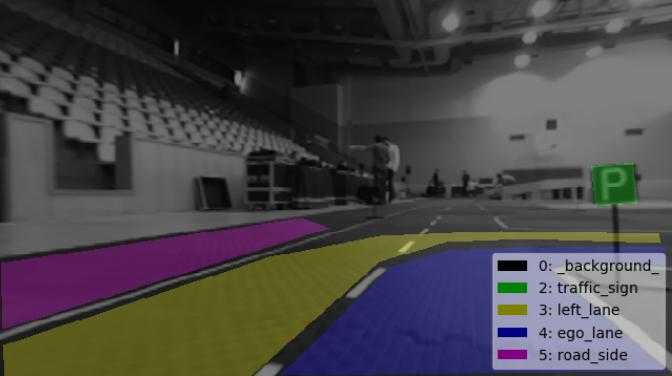
\includegraphics[width=\linewidth]{figures/course1.jpg}
    \caption{Course 1}
  \end{subfigure}
  \begin{subfigure}[b]{0.4\linewidth}
      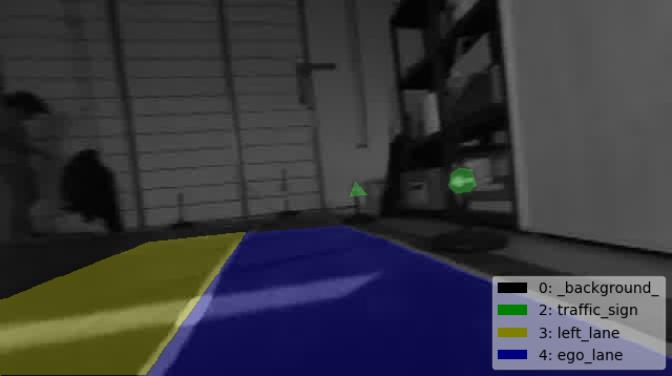
\includegraphics[width=\linewidth]{figures/course2.jpg}
    \caption{Course 2}
  \end{subfigure}
  \begin{subfigure}[b]{0.4\linewidth}
      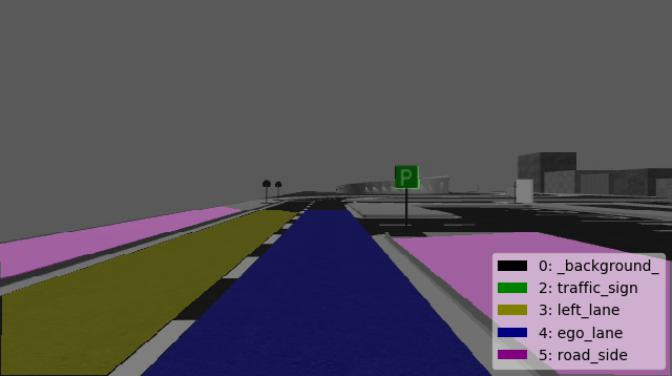
\includegraphics[width=\linewidth]{figures/course3.jpg}
    \caption{Course 3}
  \end{subfigure}
  \begin{subfigure}[b]{0.4\linewidth}
      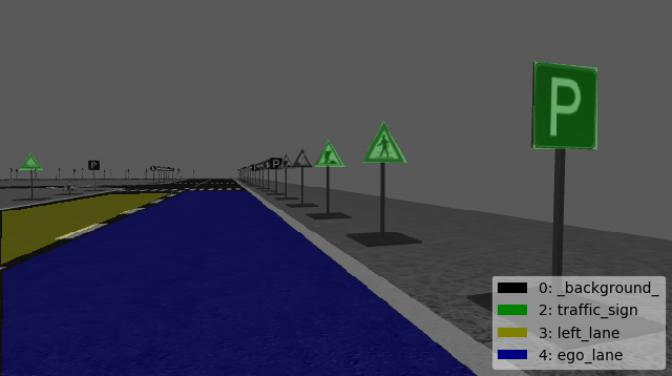
\includegraphics[width=\linewidth]{figures/course4.jpg}
    \caption{Course 4}
  \end{subfigure}
\caption{Example scenes from the courses. Course 1 is the official competition
    course. Course 2 is a small track constructed in the laboratory. Course 3
    is a simulation of Course 1. Course 4 is our simulated testing course for
    the perception component. Course 4 is not used for training the
    segmentation model.}
    \label{figure:annotated-courses}
\end{figure}

We split semantic segmentation dataset into training and testing sets as shown
in Table \ref{table:semantic-segmentation-dataset}. For classification dataset,
we started with a collection of relevant signs from existing datasets
\cite{cite11, cite12}.  Then, we expand the dataset by automatically cropping
the sign patches from the images collected from all our four courses as the car
drives itself. The new sign patches are manually arranged and merged into the
existing classification dataset. We set aside random 60 images for each class
for the testing. Details of the final classification dataset is presented in
Table \ref{table:classification-dataset}.

\begin{table}[h]
\caption{Traffic scene semantic segmentation dataset.}
\label{table:semantic-segmentation-dataset}
\resizebox{\textwidth}{!}{\begin{tabular}{||c c c||}
 \hline
 Course & Training & Testing \\ [0.5ex]
 \hline\hline
 Course 1 & 1107 & 1171 \\ 
 \hline
 Course 2 & 221 & 3 \\ 
 \hline
 Course 3 & 120 & 102 \\ 
 \hline
 Course 4 & 0 & 273 \\ [1ex]
 \hline
\end{tabular}}
\end{table}

\begin{table}[h]
\caption{Traffic sign classification dataset.}
\label{table:classification-dataset}
\resizebox{\textwidth}{!}{\begin{tabular}{||c c c c||}
 \hline
 Class & Training & Testing & Auto-cropped \\ [0.5ex]
 \hline\hline
 CrossRoad & 704 & 89 & 470 \\ 
 \hline
 KeepLeft & 832 & 83 & 582 \\ 
 \hline
 LooseRoad & 473 & 60 & 533\\ 
 \hline
 NoEntry & 502 & 83 & 306 \\ 
 \hline
 Parking & 497 & 90 & 237 \\ 
 \hline
 ParkingSlot & 1728 & 60 & 1788 \\ 
 \hline
 RoadWork & 1728 & 86 & 224 \\ 
 \hline
 StraightOrRight & 1105 & 89 & 847 \\ 
 \hline
 TrafficLightGreen & 422 & 76 & 192 \\ 
 \hline
 TrafficLightRed & 1145 & 72 & 1093 \\ 
 \hline
 TurnLeft & 811 & 93 & 496 \\
 \hline
 Negative & 963 & 60 & 1023 \\ [1ex]
 \hline
\end{tabular}}
\end{table}

\section{Perception Evaluation}
For the performance evaluation of our semantic segmentation model, we use
intersection over union (IoU), precision, recall and F1-score metrics defined
as follows:

\begin{equation}
    IoU = \frac{TP}{TP + FP + FN},
\label{eq:iou}
\end{equation}


\begin{equation}
    Precision = \frac{TP}{TP + FP},
\label{eq:precision}
\end{equation}


\begin{equation}
    Recall = \frac{TP}{TP + FN},
\label{eq:recall}
\end{equation}

\begin{equation}
    F1 = \frac{2.Precision.Recall}{Precision + Recall},
\label{eq:F1}
\end{equation}

where TP, FP, and FN represent the number of true positives, false positives
and false negatives, respecetively.

Once we trained the segmentation model with the whole training set given in
Table \ref{table:semantic-segmentation-dataset}, we test it against first
Course 4 only then the whole test set in Table
\ref{table:semantic-segmentation-dataset}. Note that the model does not see
Course 4 images during training. Table \ref{table:segmentation-metrics1} and
Table \ref{table:segmentation-metrics2} present the evalutation metrics for
Course 4 only and the whole test set, respectively.

\begin{table}[h]
\caption{Semantic segmentation evalutation metrics for the Course 4 test only.}
\label{table:segmentation-metrics1}
\resizebox{\textwidth}{!}{\begin{tabular}{||c c c c c||}
 \hline
 Class & IoU & Precision & Recall & F1-score \\ [0.5ex]
 \hline\hline
 Ego Lane & 81.42\% & 95.00\% & 84.30\% & 89.32\% \\ 
 \hline
 Right Lane & 34.36\% & 61.87\% & 51.96\% & 56.49\% \\ 
 \hline
 Left Lane & 54.82\% & 63.23\% & 82.38\% & 71.55\% \\ 
 \hline
 Traffic Sign & 39.66\% & 67.21\% & 50.70\% & 57.80\% \\ [1ex]
 \hline
\end{tabular}}
\end{table}

\begin{table}[h]
\caption{Semantic segmentation evalutation metrics for the whole test set.}
\label{table:segmentation-metrics2}
\resizebox{\textwidth}{!}{\begin{tabular}{||c c c c c||}
 \hline
 Class & IoU & Precision & Recall & F1-score \\ [0.5ex]
 \hline\hline
 Ego Lane & 82.27\% & 89.35\% & 88.86\% & 89.10\% \\ 
 \hline
 Right Lane & 39.02\% & 55.07\% & 65.90\% & 60.00\% \\ 
 \hline
 Left Lane & 68.96\% & 76.41\% & 88.16\% & 81.86\% \\ 
 \hline
 Traffic Sign & 36.08\% & 70.17\% & 43.82\% & 53.95\% \\ [1ex]
 \hline
\end{tabular}}
\end{table}

For the first classification test, we excluded our auto-cropped sign images
from both training and test sets given in Table
\ref{table:classification-dataset}.  With the merged existing sign recognition
datasets, we achieved 99.54\% accuracy.  Table
\ref{table:classification-metrics1} presents the detailed metrics of this test
run.


\begin{table}[h]
\caption{Traffic sign classification test on the merged existing test sets.}
\label{table:classification-metrics1}
\resizebox{\textwidth}{!}{\begin{tabular}{||c c c c||}
 \hline
 Class             & Precision & Recall    & F1-score \\ [0.5ex]
 \hline\hline
 CrossRoad         & 100.00\%  & 100.00\%   &  100.00\% \\ 
 \hline
 KeepLeft          & 100.00\%  & 100.00\%  & 100.00\% \\ 
 \hline
 LooseRoad         &   N/A     &  N/A      &  N/A     \\ 
 \hline
 NoEntry           & 100.00\%  & 100.00\%   &  100.00\% \\ 
 \hline
 Parking           & 100.00\%  & 100.00\%   &  100.00\% \\ 
 \hline
 ParkingSlot       &   N/A     & N/A       &    N/A   \\ 
 \hline
 RoadWork          & 100.00\%   & 100.00\%  &  100.00\% \\ 
 \hline
 StraightOrRight   & 100.00\%  & 100.00\%   & 100.00\%  \\ 
 \hline
 TrafficLightGreen & 100.00\%   & 100.00\%  & 100.00\%  \\ 
 \hline
 TrafficLightRed   & 92.30\%  & 100.00\%   & 96.00\%  \\ 
 \hline
 TurnLeft          & 100.00\%   & 96.97\%   & 98.46\%  \\
 \hline
 Negative          & N/A       & N/A       & N/A      \\ [1ex]
 \hline
\end{tabular}}
\end{table}

Then, we trained and tested the model on the whole classification dataset and
this time achieved 97.37\% accuracy. Table \ref{table:classification-metrics2}
gives the metrics for the second classification test.

\begin{table}[h]
\caption{Traffic sign classification test on the whole test set.}
\label{table:classification-metrics2}
\resizebox{\textwidth}{!}{\begin{tabular}{||c c c c||}
 \hline
 Class             & Precision & Recall    & F1-score \\ [0.5ex]
 \hline\hline
 CrossRoad         & 96.00\%   & 97.75\%   &  97.21\% \\ 
 \hline
 KeepLeft          & 100.00\%  & 98.80\%   & 100.00\% \\ 
 \hline
 LooseRoad         & 98.36\%   & 100.00\%  &  99.17\% \\ 
 \hline
 NoEntry           & 95.29\%   & 97.59\%   &  96.43\% \\
 \hline
 Parking           & 97.80\%  & 98.89\%   &  98.34\% \\ 
 \hline
 ParkingSlot       & 89.23\%   & 96.97\%  &  92.80\%  \\ 
 \hline
 RoadWork          & 96.51\%   & 96.51\%  &  96.51\% \\ 
 \hline
 StraightOrRight   & 100.00\%  & 98.87\%   & 99.43\%  \\ 
 \hline
 TrafficLightGreen & 98.67\%   & 97.37\%  & 98.01\%  \\ 
 \hline
 TrafficLightRed   & 100.00\%  & 97.56\%   & 98.76\%  \\ 
 \hline
 TurnLeft          & 96.74\%   & 95.70\%   & 96.22\%  \\
 \hline
 Negative          & 98.21\%   & 91.67\%   & 94.83\%  \\ [1ex]
 \hline
\end{tabular}}
\end{table}

\section{Driving Tasks}

\begin{figure}[h]
  \centering
  \begin{subfigure}[b]{0.45\linewidth}
      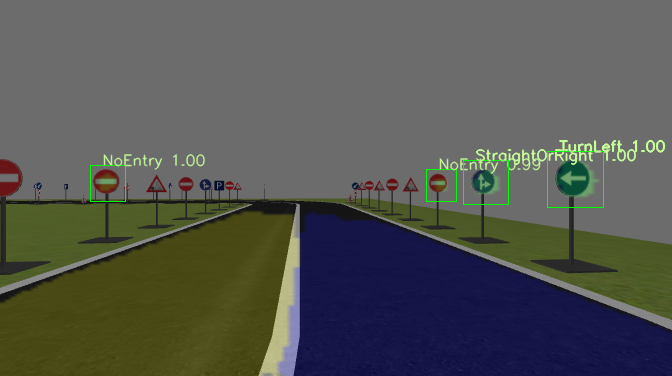
\includegraphics[width=\linewidth]{figures/experiments/lane-following-img.png}
  \end{subfigure}
  \begin{subfigure}[b]{0.45\linewidth}
      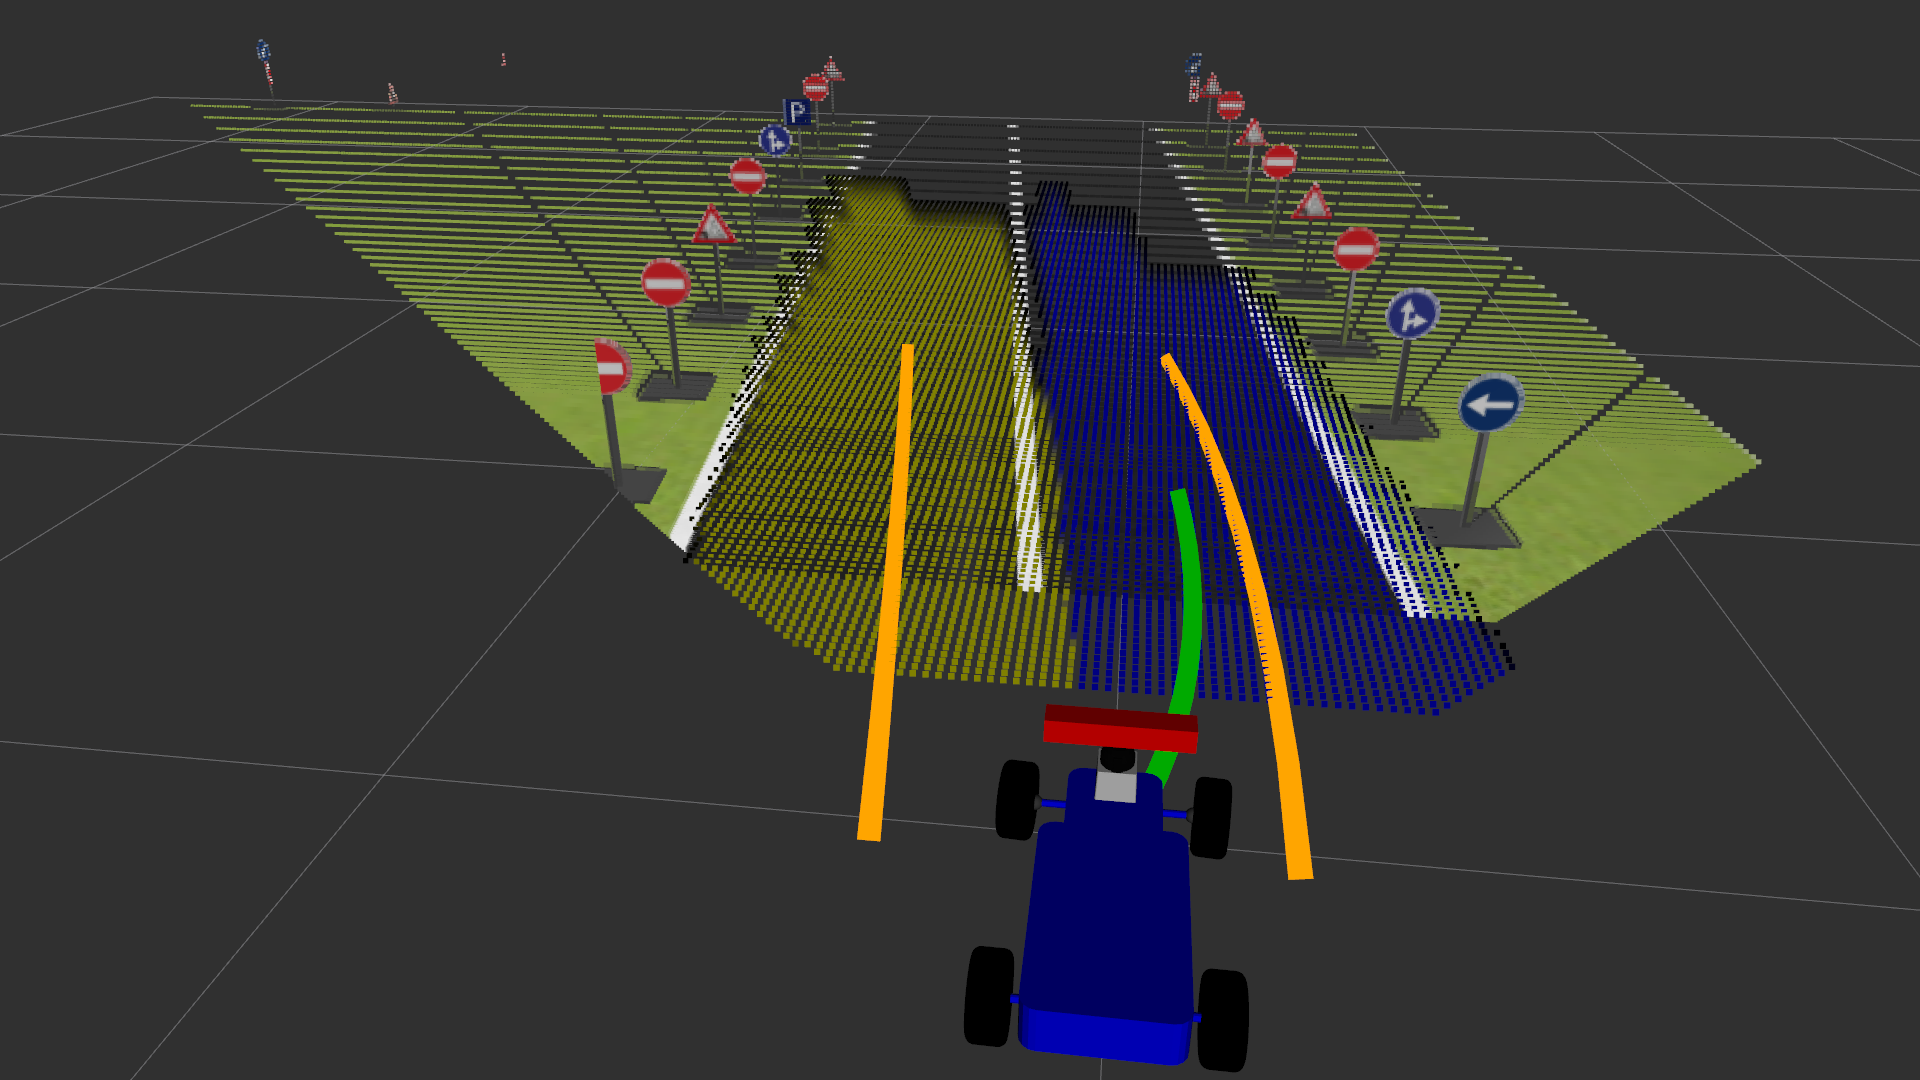
\includegraphics[width=\linewidth]{figures/experiments/lane-following-pc.png}
  \end{subfigure}
  \begin{subfigure}[b]{0.45\linewidth}
      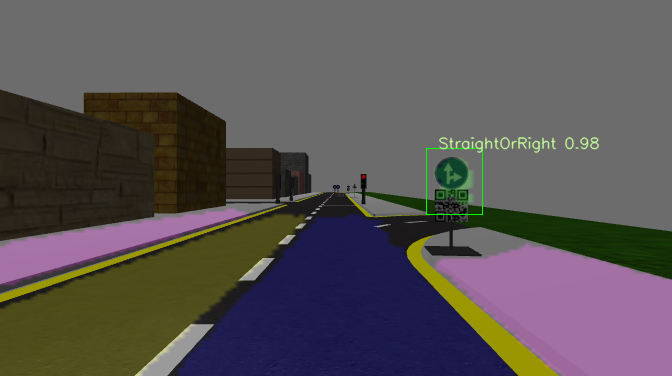
\includegraphics[width=\linewidth]{figures/experiments/straight-or-right-img.png}
  \end{subfigure}
  \begin{subfigure}[b]{0.45\linewidth}
      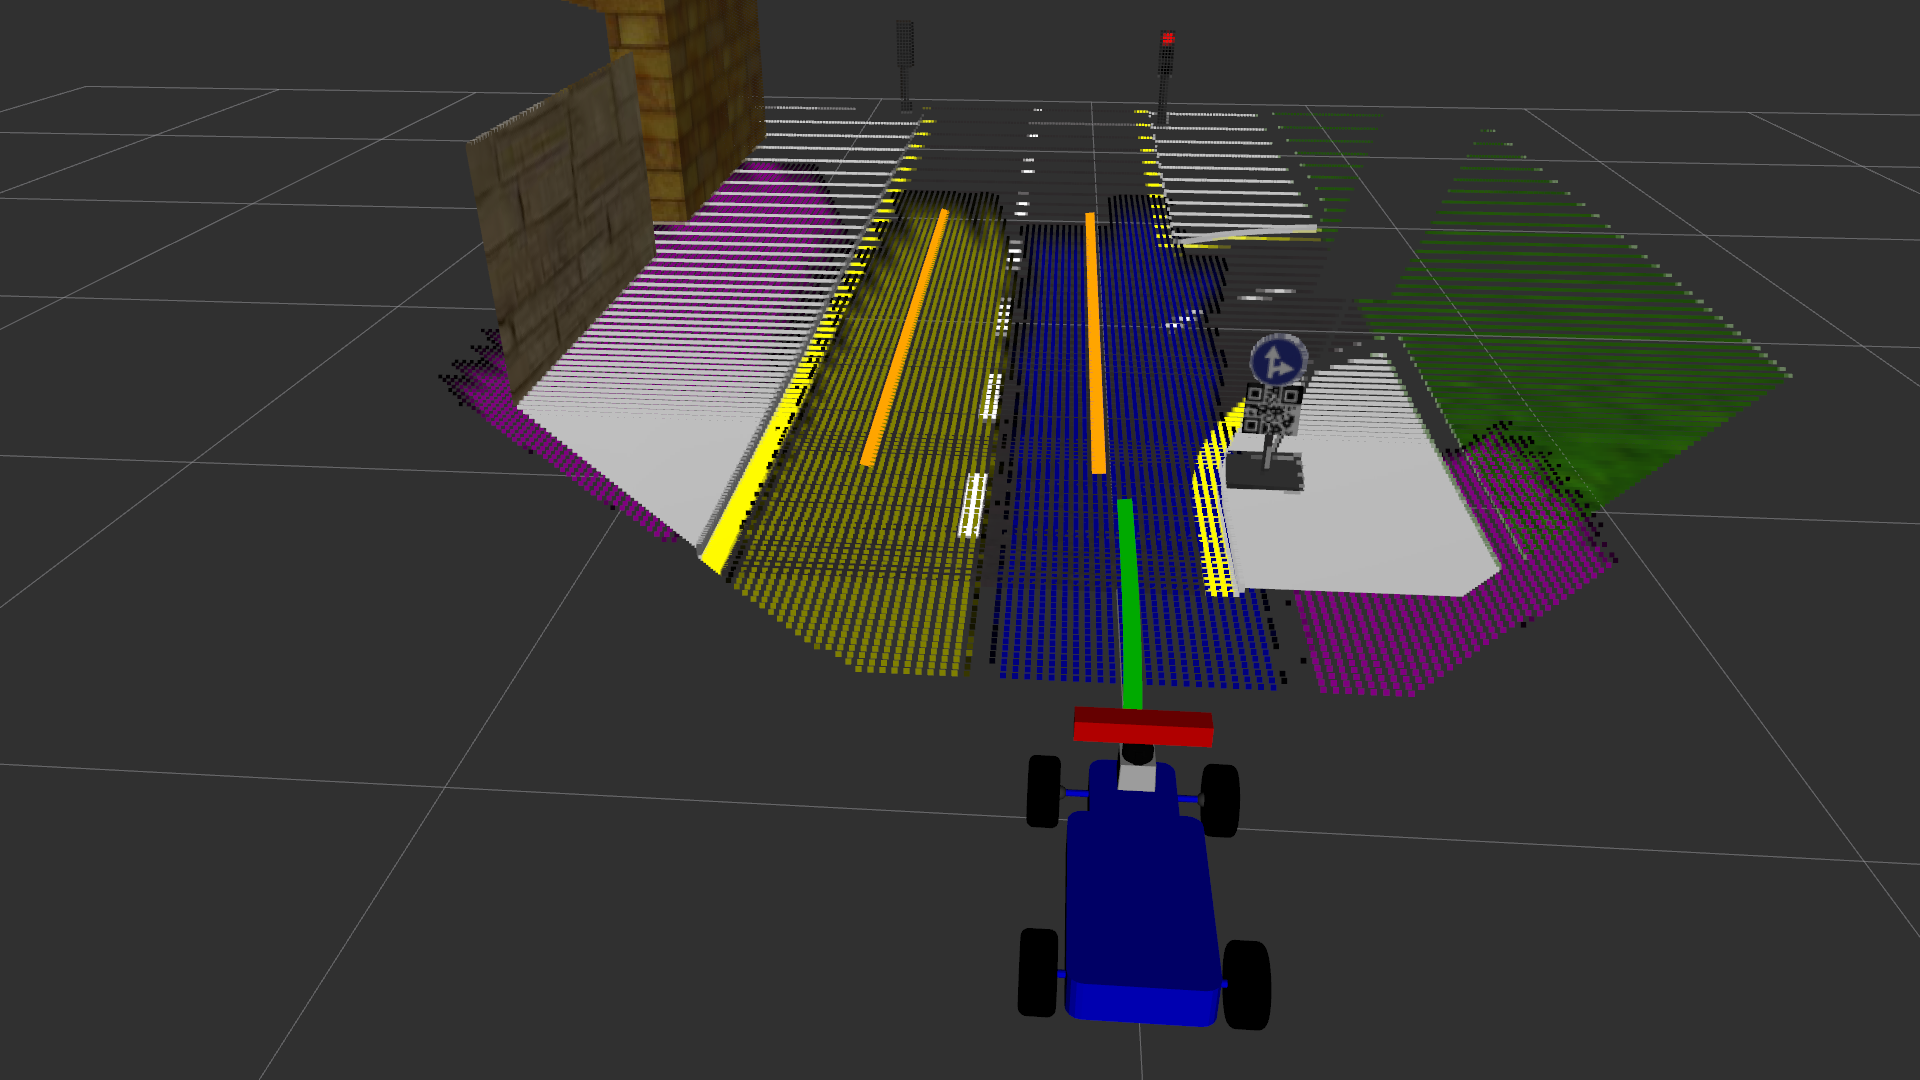
\includegraphics[width=\linewidth]{figures/experiments/straight-or-right-pc.png}
  \end{subfigure}
  \begin{subfigure}[b]{0.45\linewidth}
      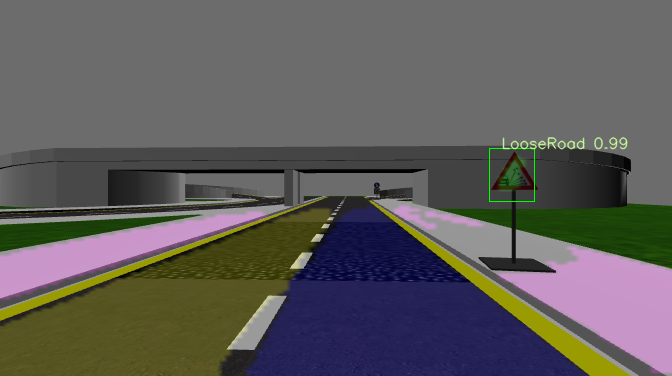
\includegraphics[width=\linewidth]{figures/experiments/loose-road-img.png}
  \end{subfigure}
  \begin{subfigure}[b]{0.45\linewidth}
      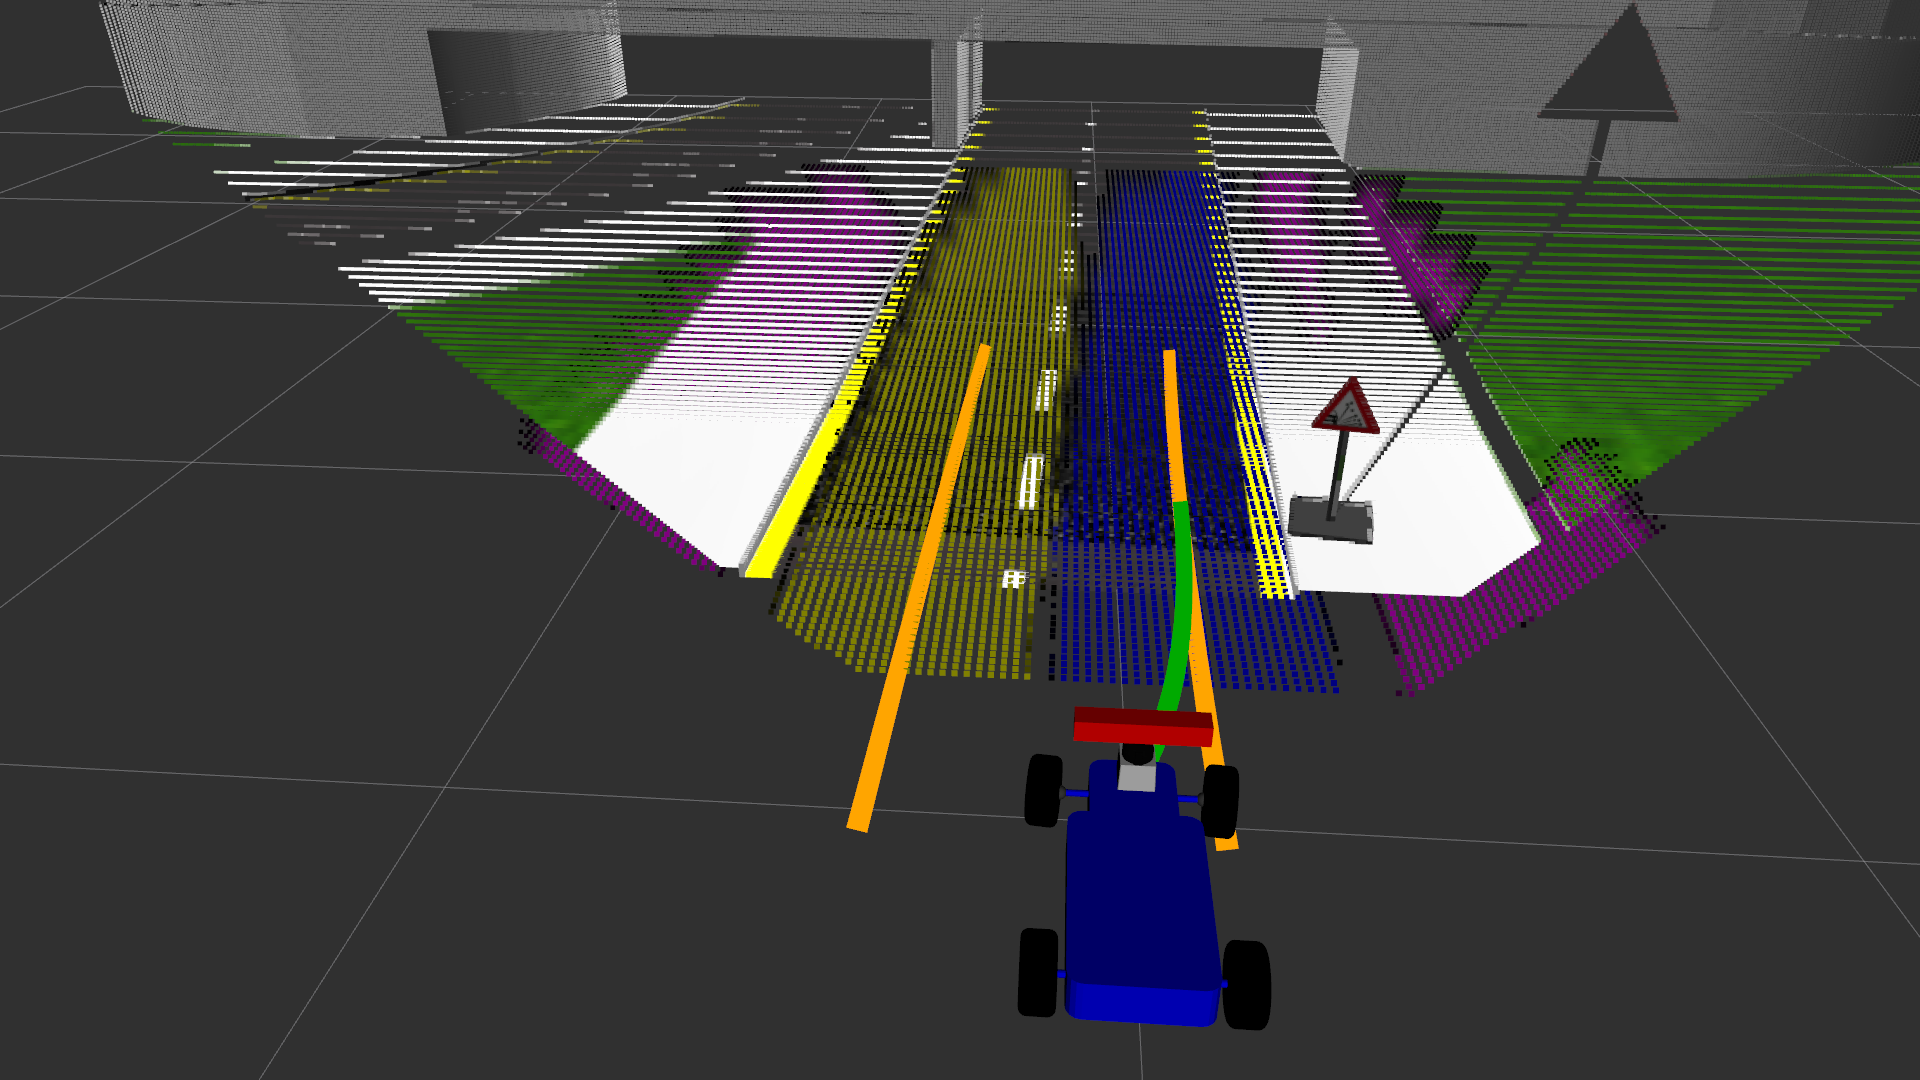
\includegraphics[width=\linewidth]{figures/experiments/loose-road-pc.png}
  \end{subfigure}
  \caption{Experiments.}
  \label{figure:normal-driving}
\end{figure}

\begin{figure}[h]
  \centering
  \begin{subfigure}[b]{0.45\linewidth}
      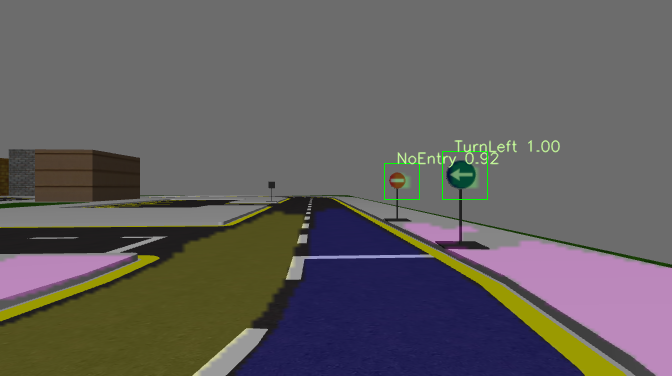
\includegraphics[width=\linewidth]{figures/experiments/turn-left-img.png}
  \end{subfigure}
  \begin{subfigure}[b]{0.45\linewidth}
      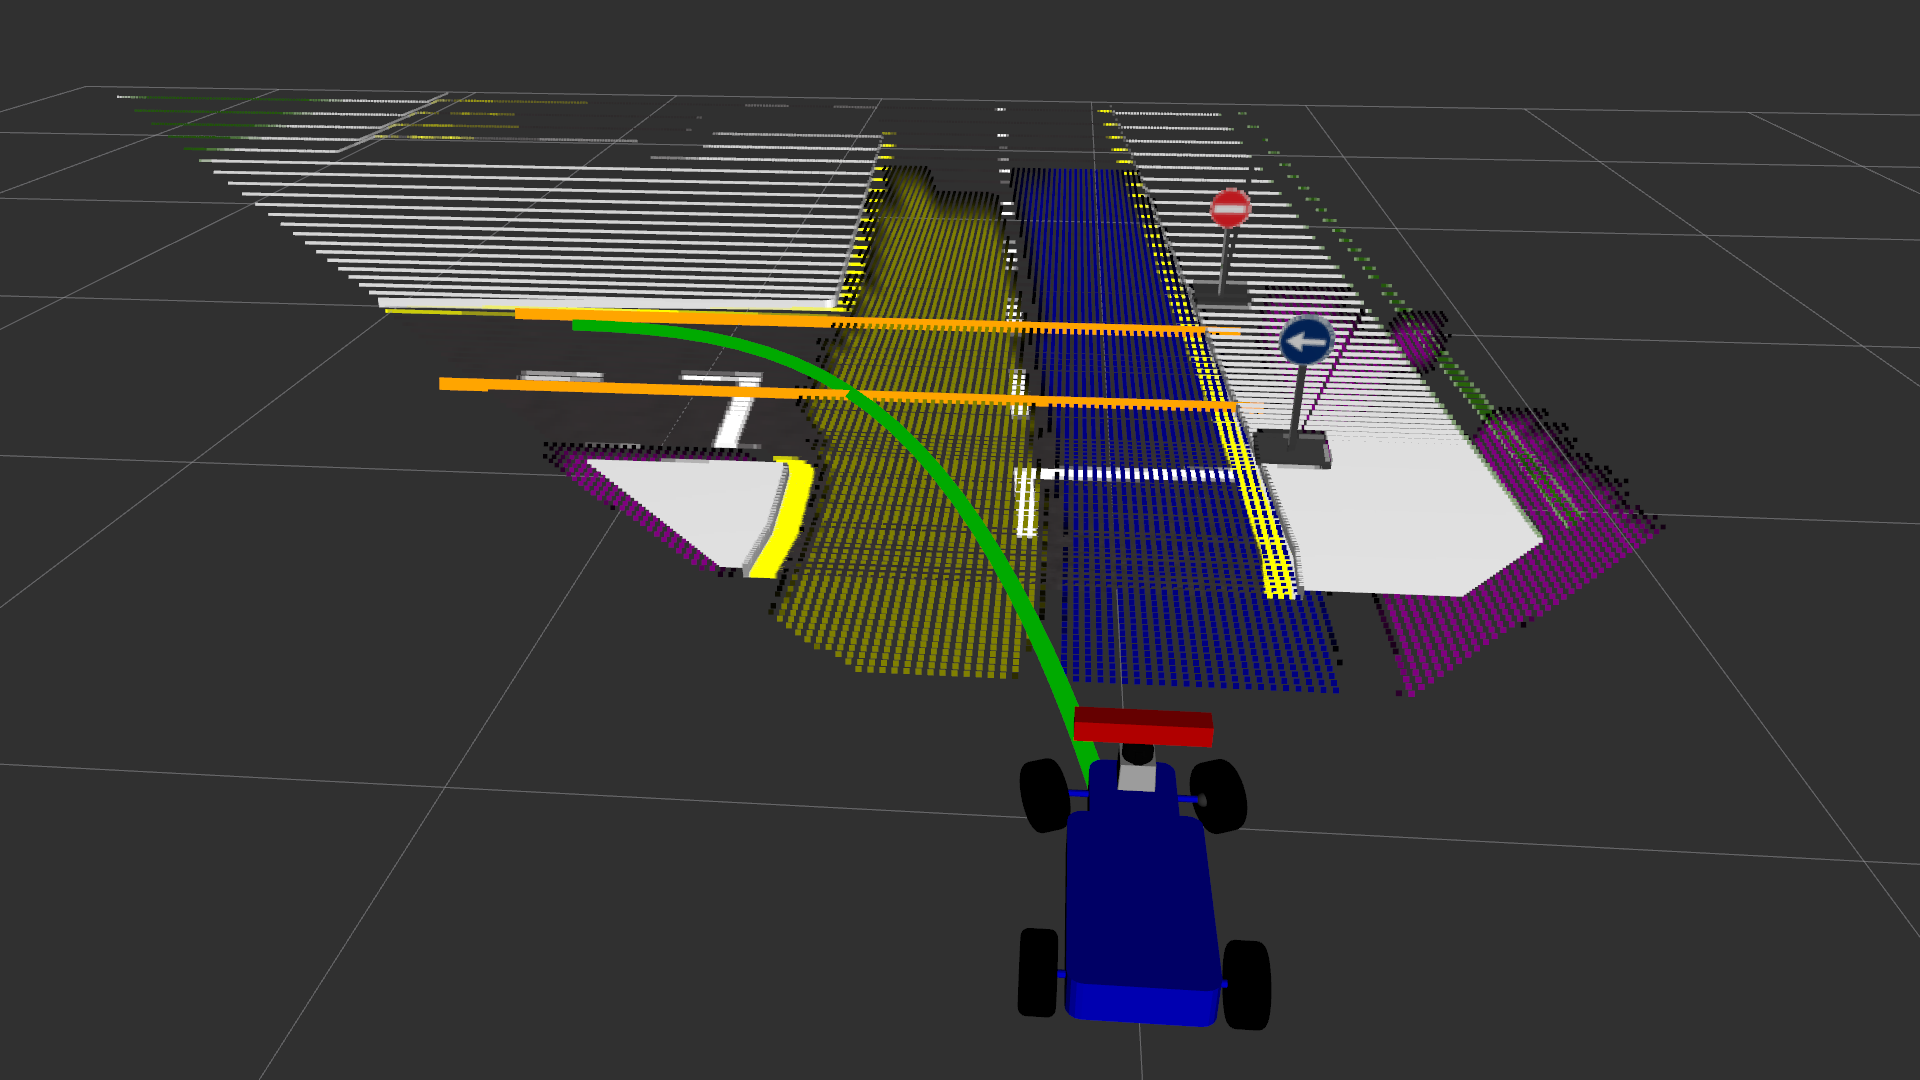
\includegraphics[width=\linewidth]{figures/experiments/turn-left-pc.png}
  \end{subfigure}
  \begin{subfigure}[b]{0.45\linewidth}
      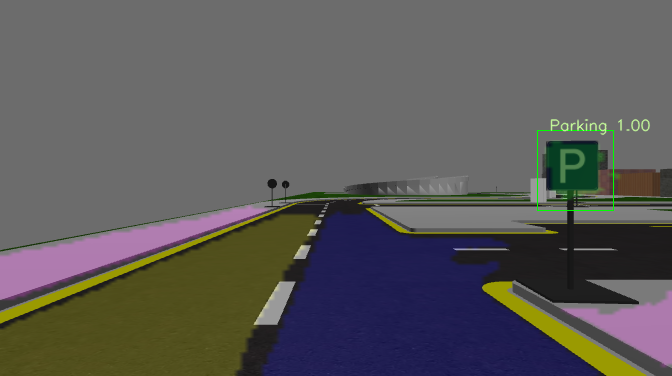
\includegraphics[width=\linewidth]{figures/experiments/parking-img.png}
  \end{subfigure}
  \begin{subfigure}[b]{0.45\linewidth}
      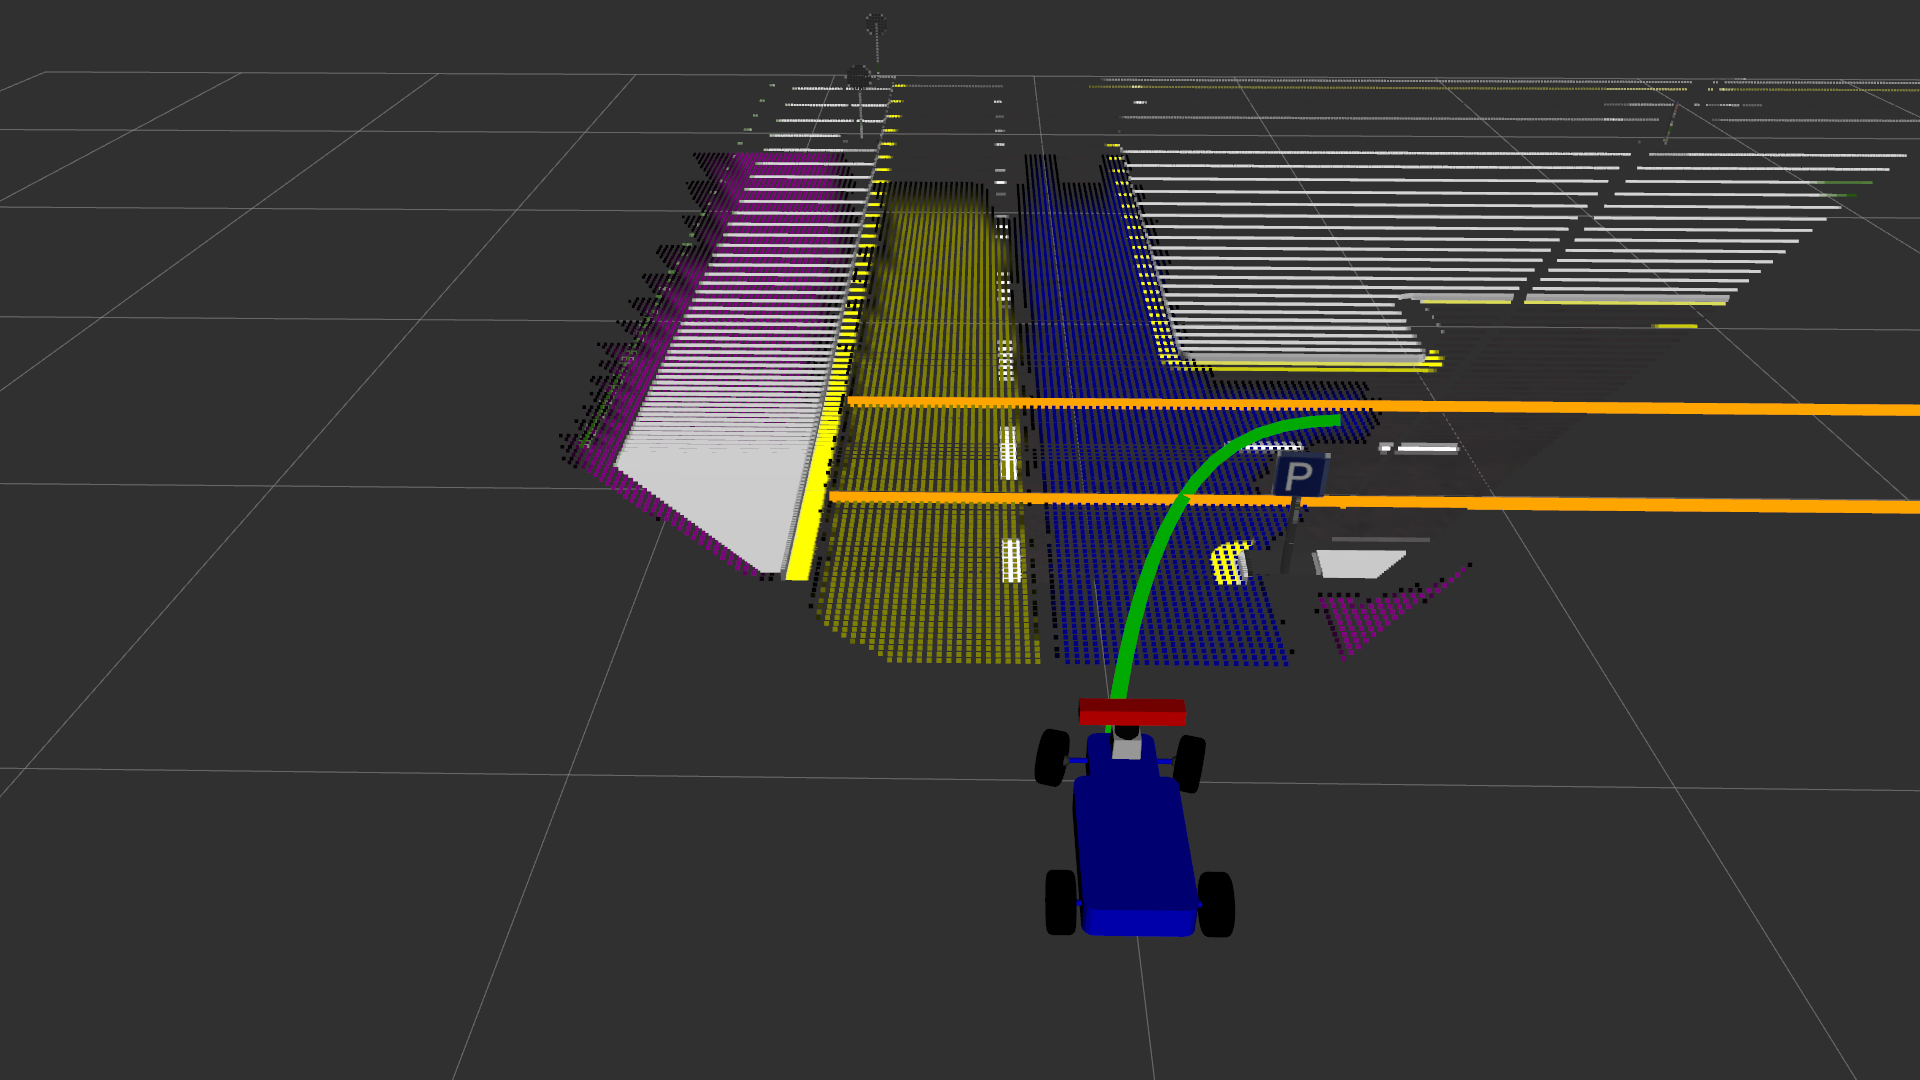
\includegraphics[width=\linewidth]{figures/experiments/parking-pc.png}
  \end{subfigure}
  \caption{Experiments.}
  \label{figure:sharp-turns}
\end{figure}

\begin{figure}[h]
  \centering
  \begin{subfigure}[b]{0.45\linewidth}
      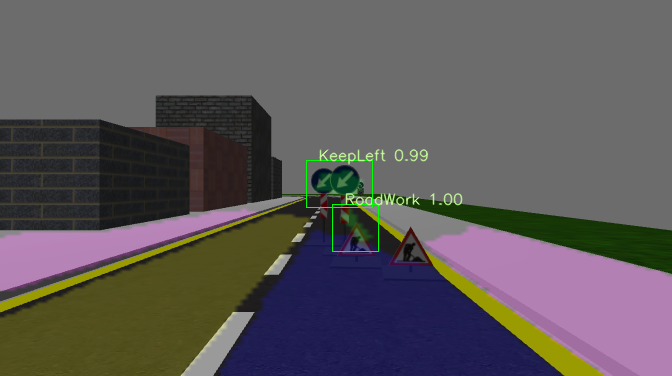
\includegraphics[width=\linewidth]{figures/experiments/construction-zone-img.png}
  \end{subfigure}
  \begin{subfigure}[b]{0.45\linewidth}
      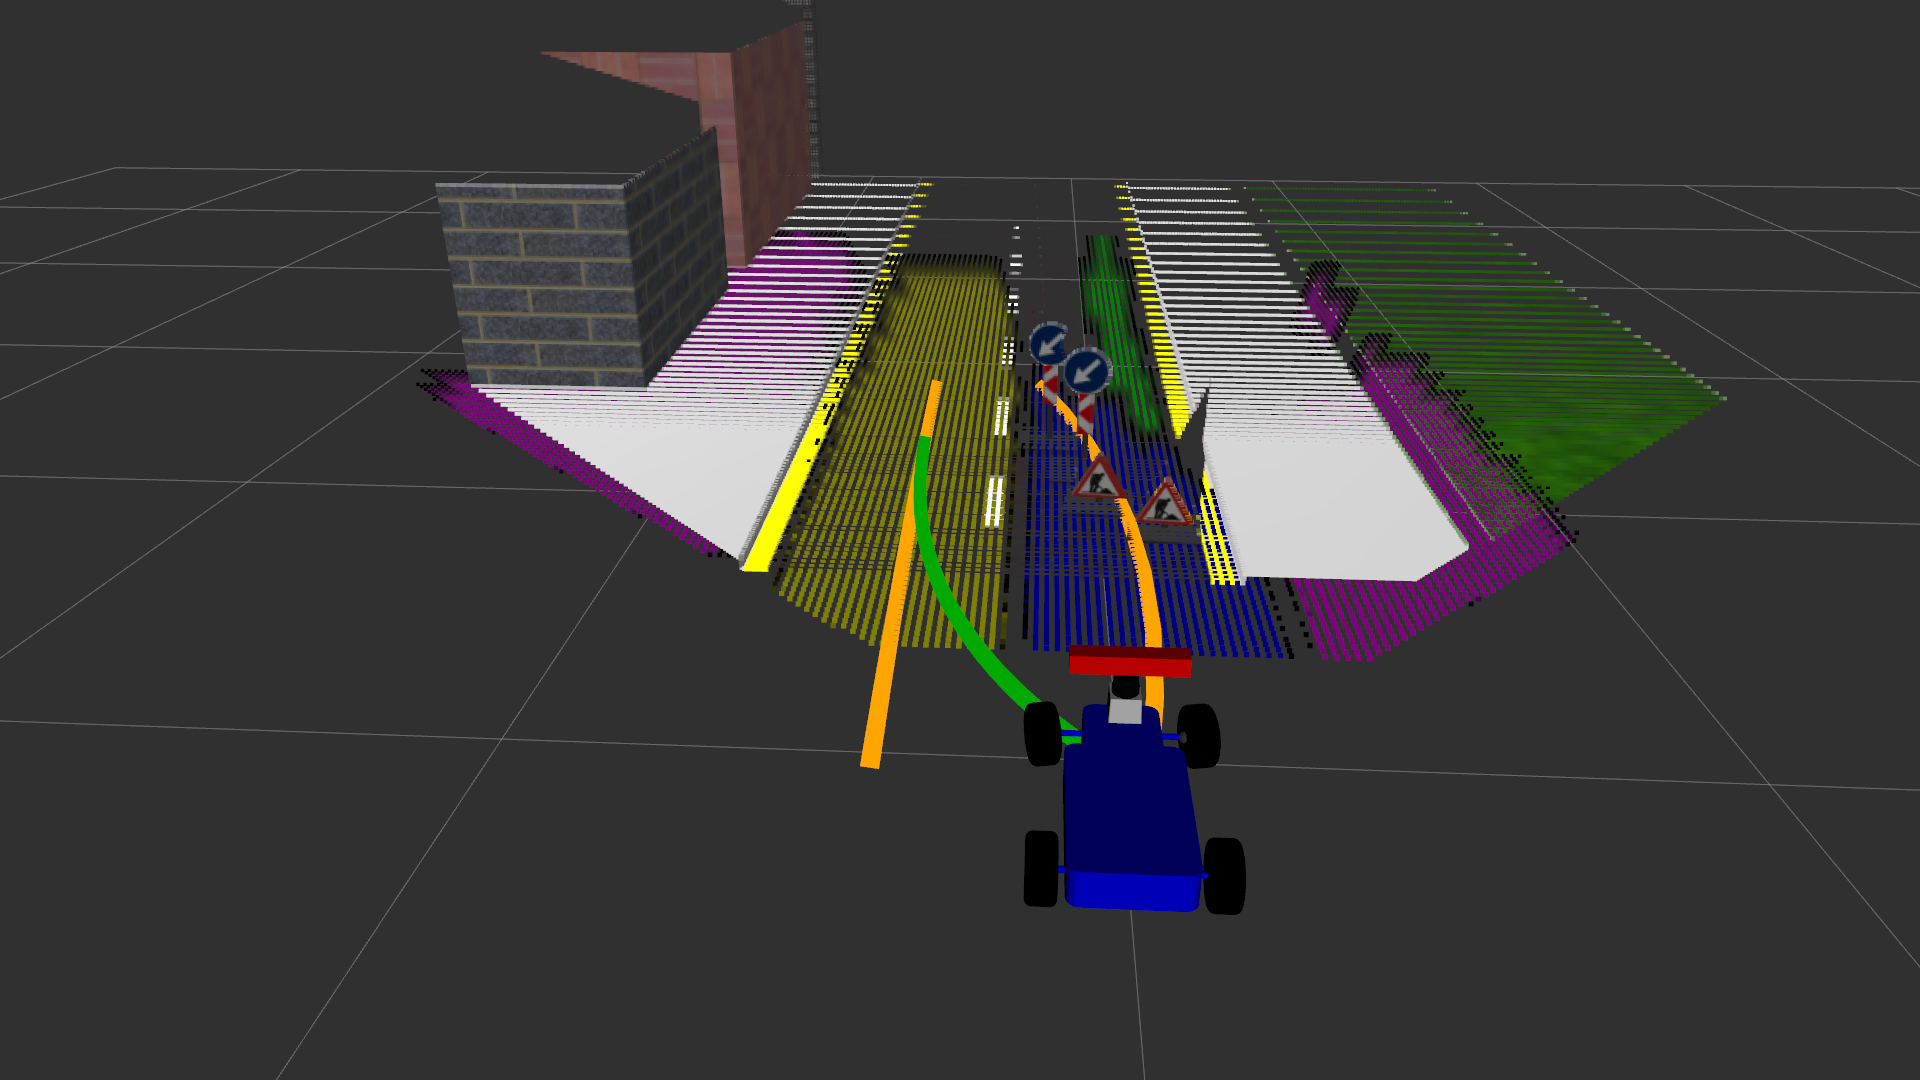
\includegraphics[width=\linewidth]{figures/experiments/construction-zone-pc.png}
  \end{subfigure}
  \begin{subfigure}[b]{0.45\linewidth}
      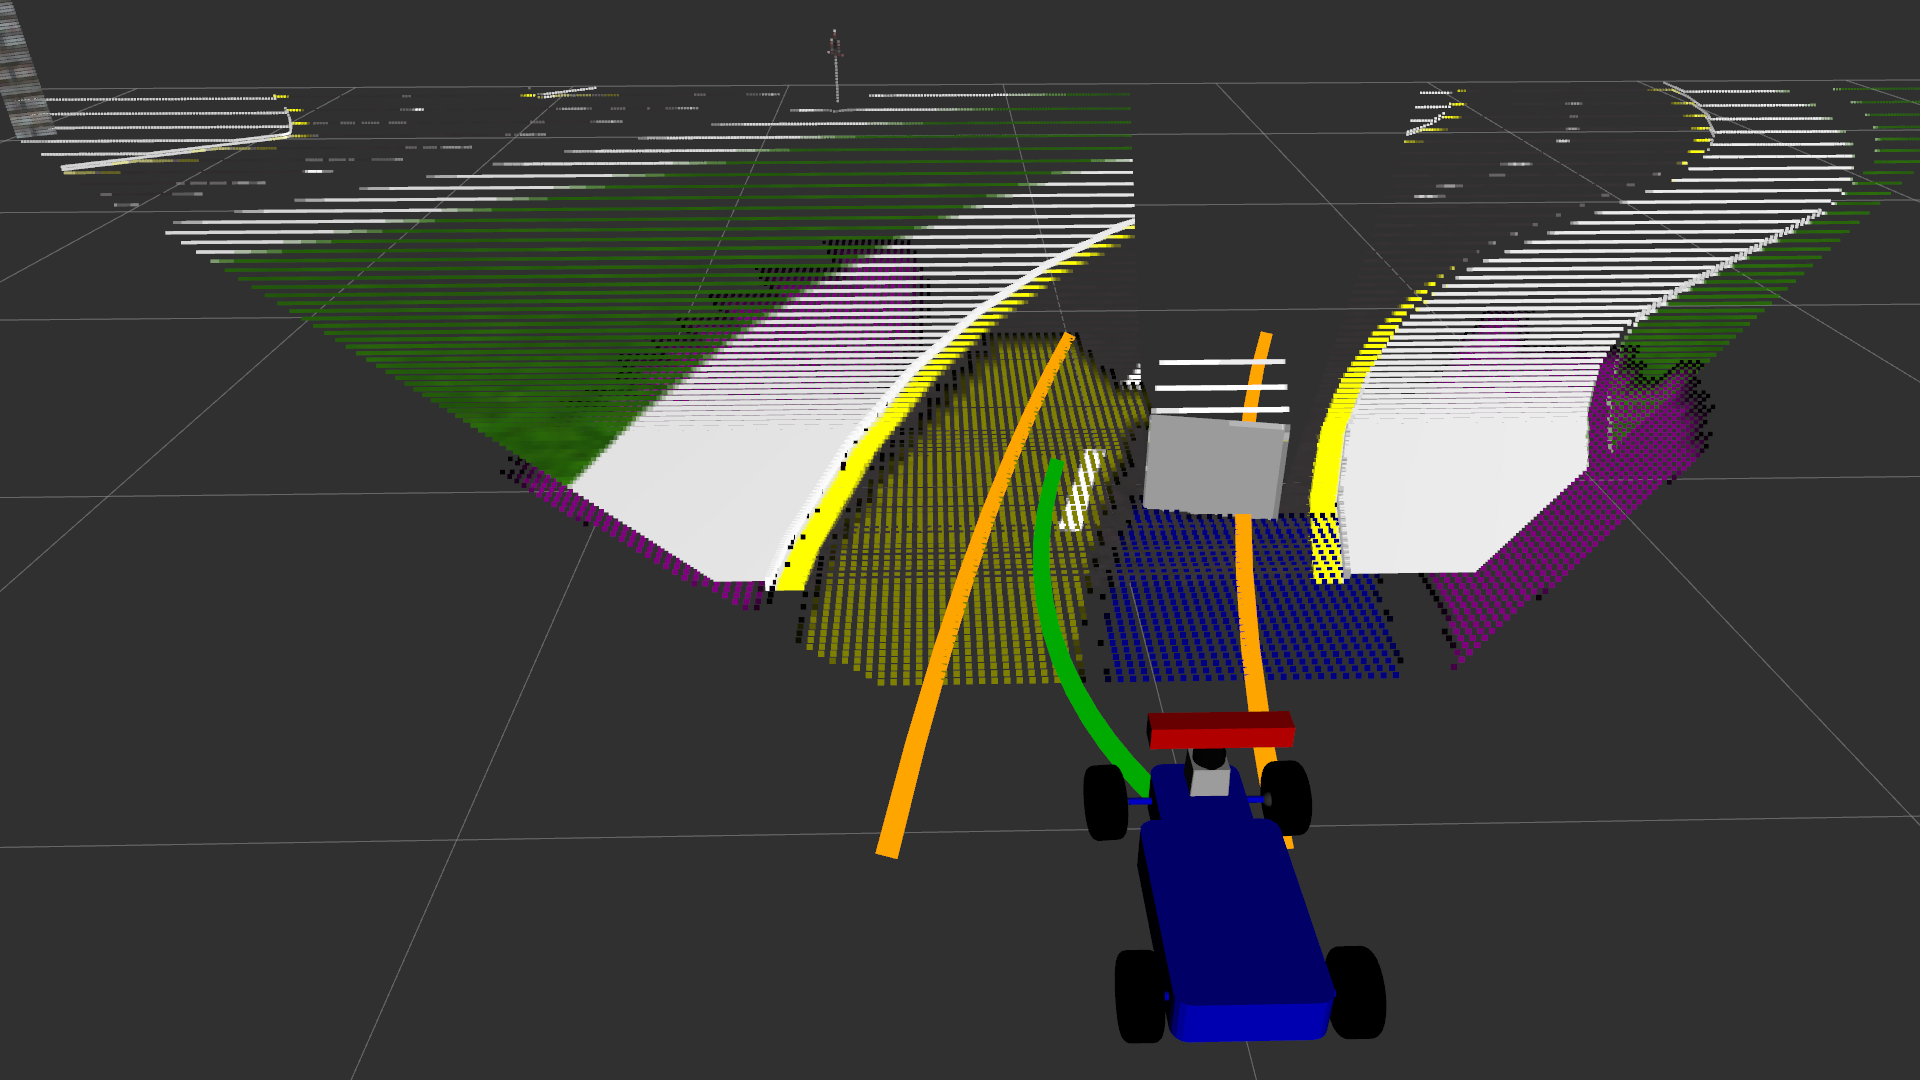
\includegraphics[width=\linewidth]{figures/experiments/overtaking1-pc.png}
  \end{subfigure}
  \begin{subfigure}[b]{0.45\linewidth}
      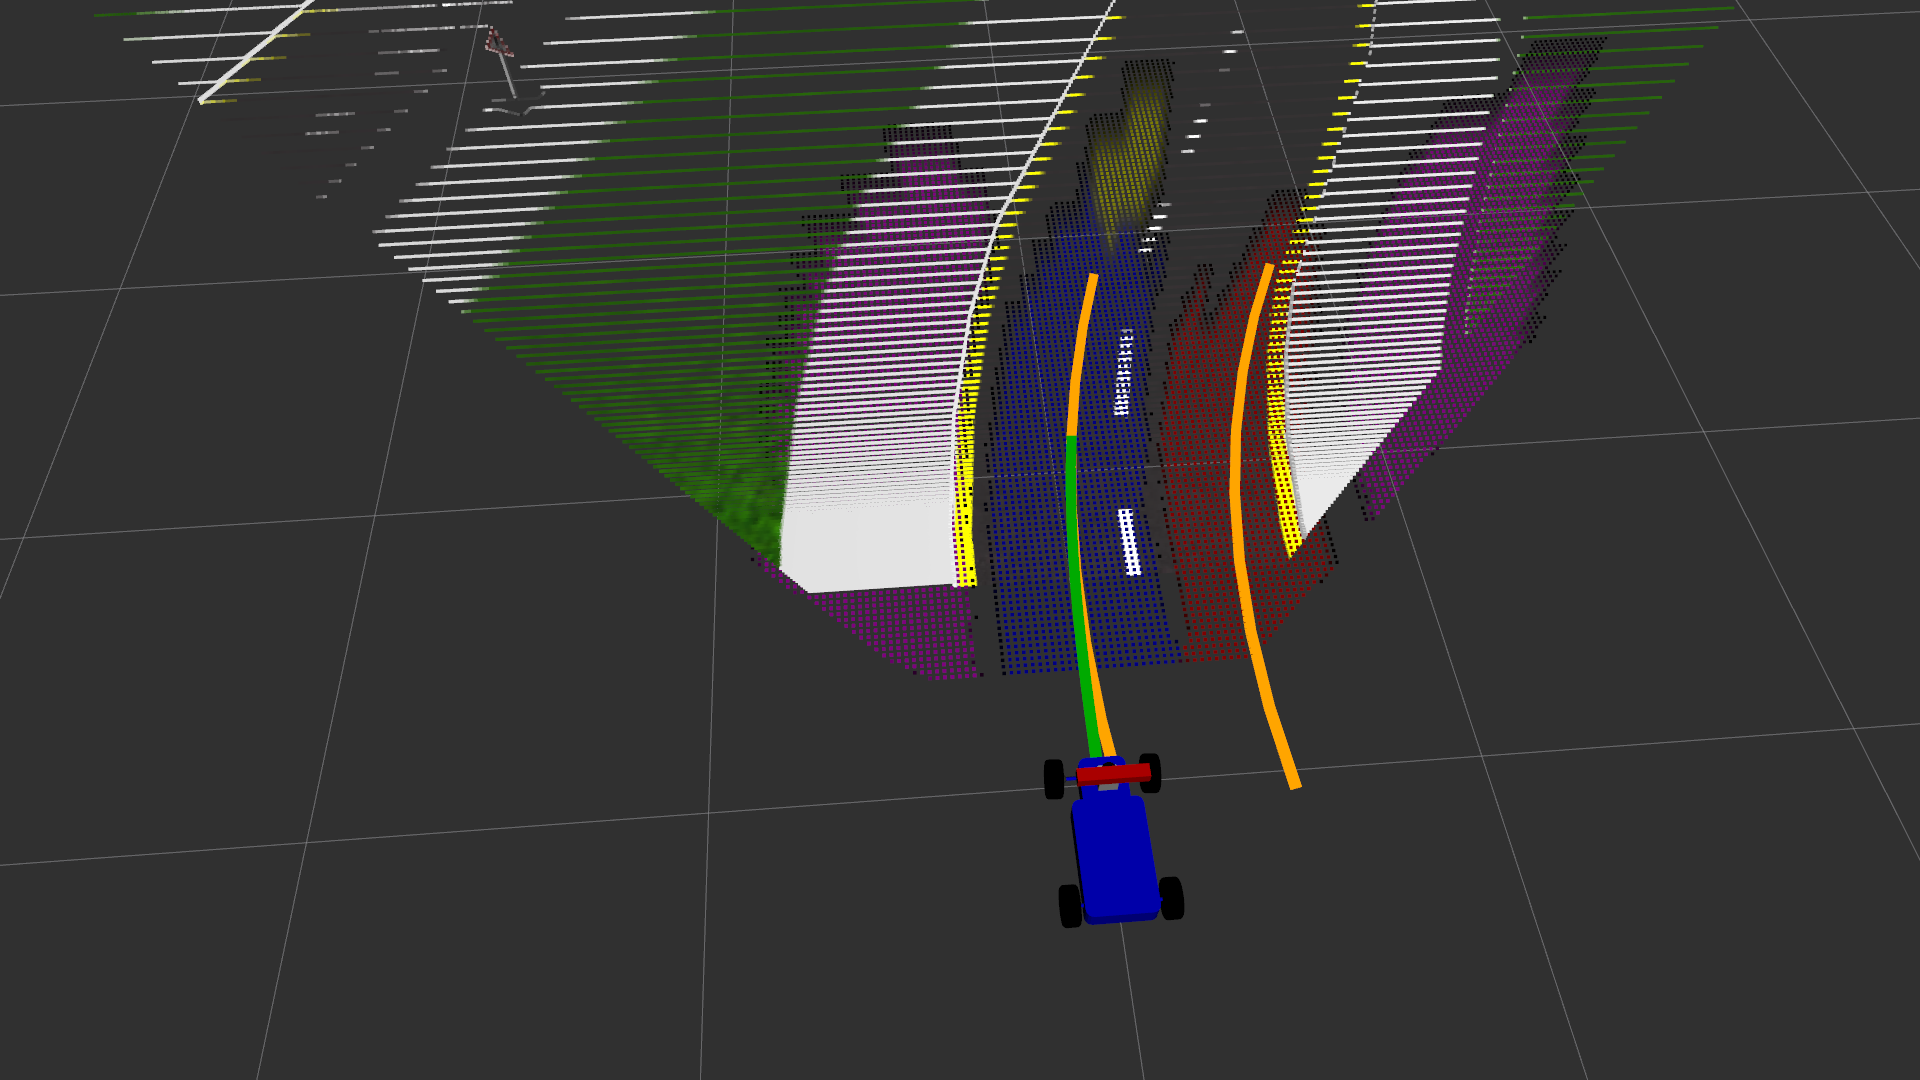
\includegraphics[width=\linewidth]{figures/experiments/overtaking2-pc.png}
  \end{subfigure}
  \begin{subfigure}[b]{0.45\linewidth}
      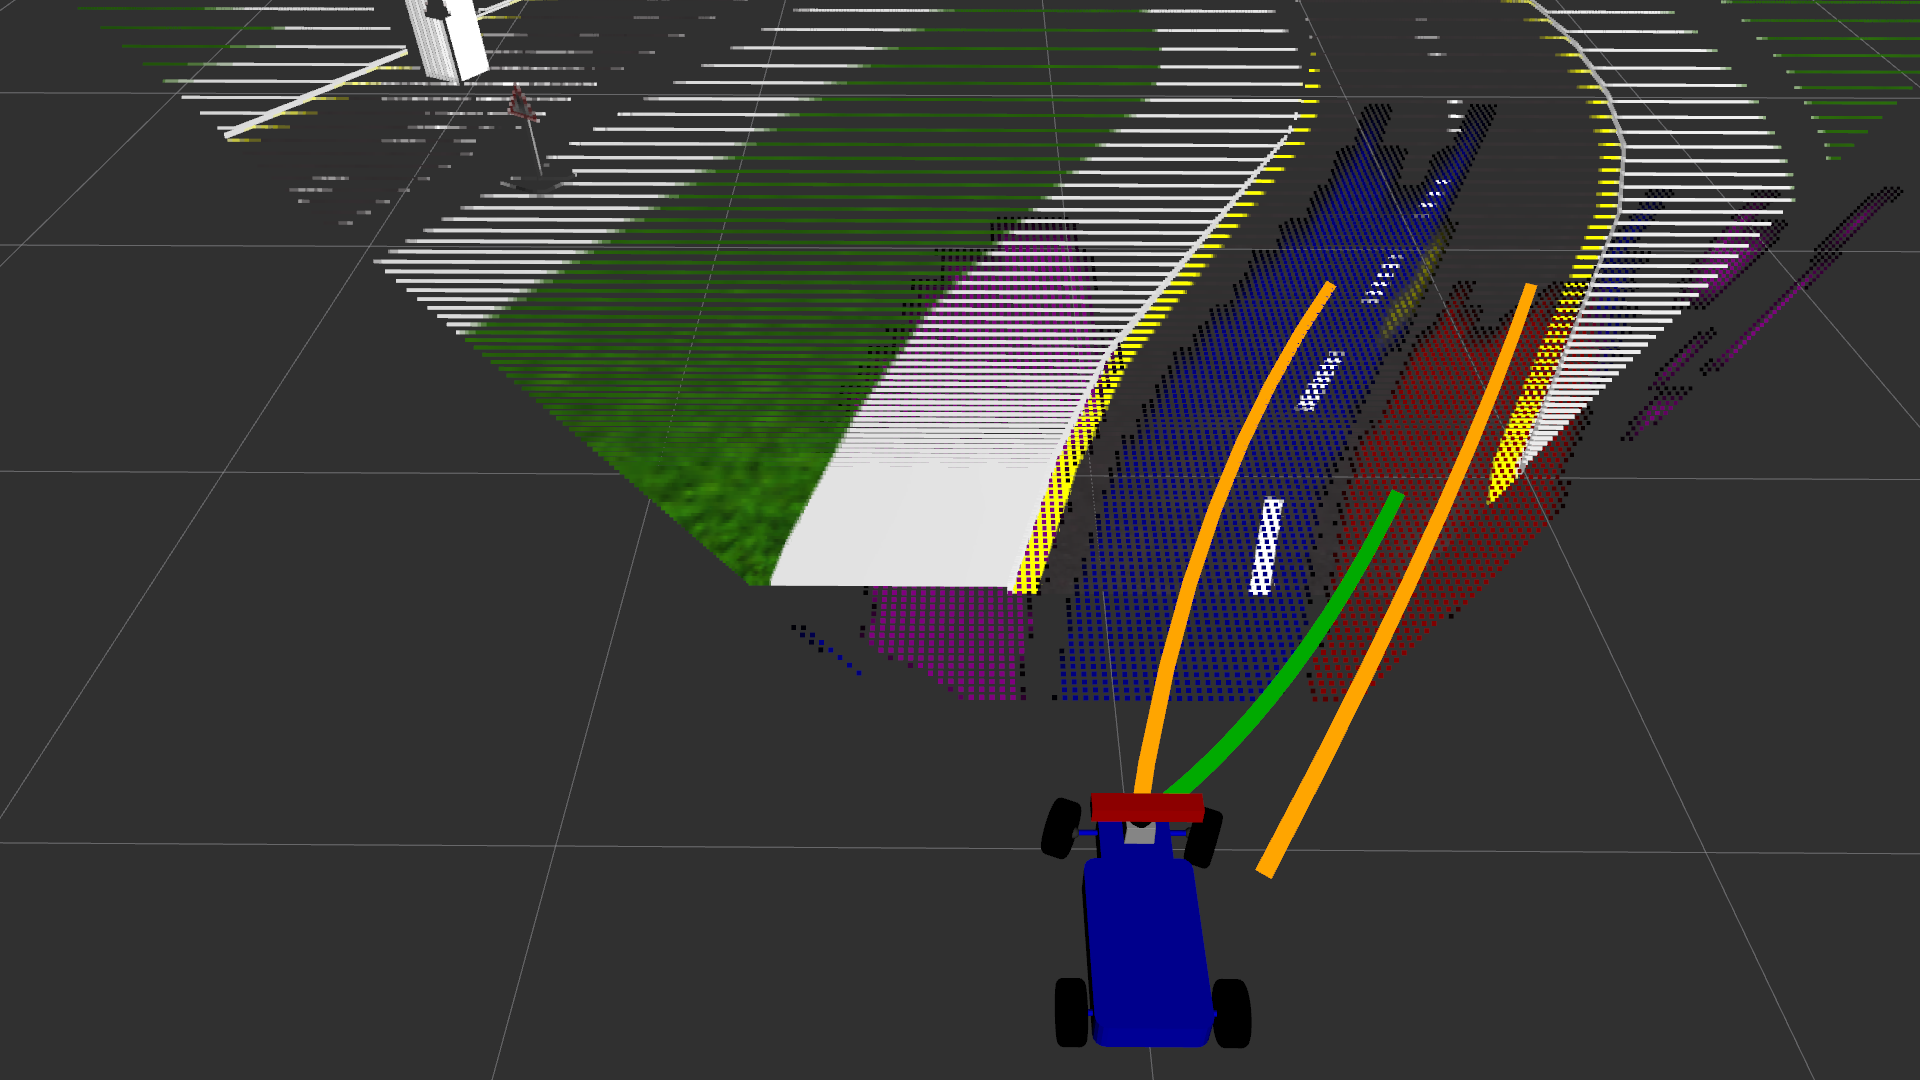
\includegraphics[width=\linewidth]{figures/experiments/overtaking3-pc.png}
  \end{subfigure}
  \begin{subfigure}[b]{0.45\linewidth}
      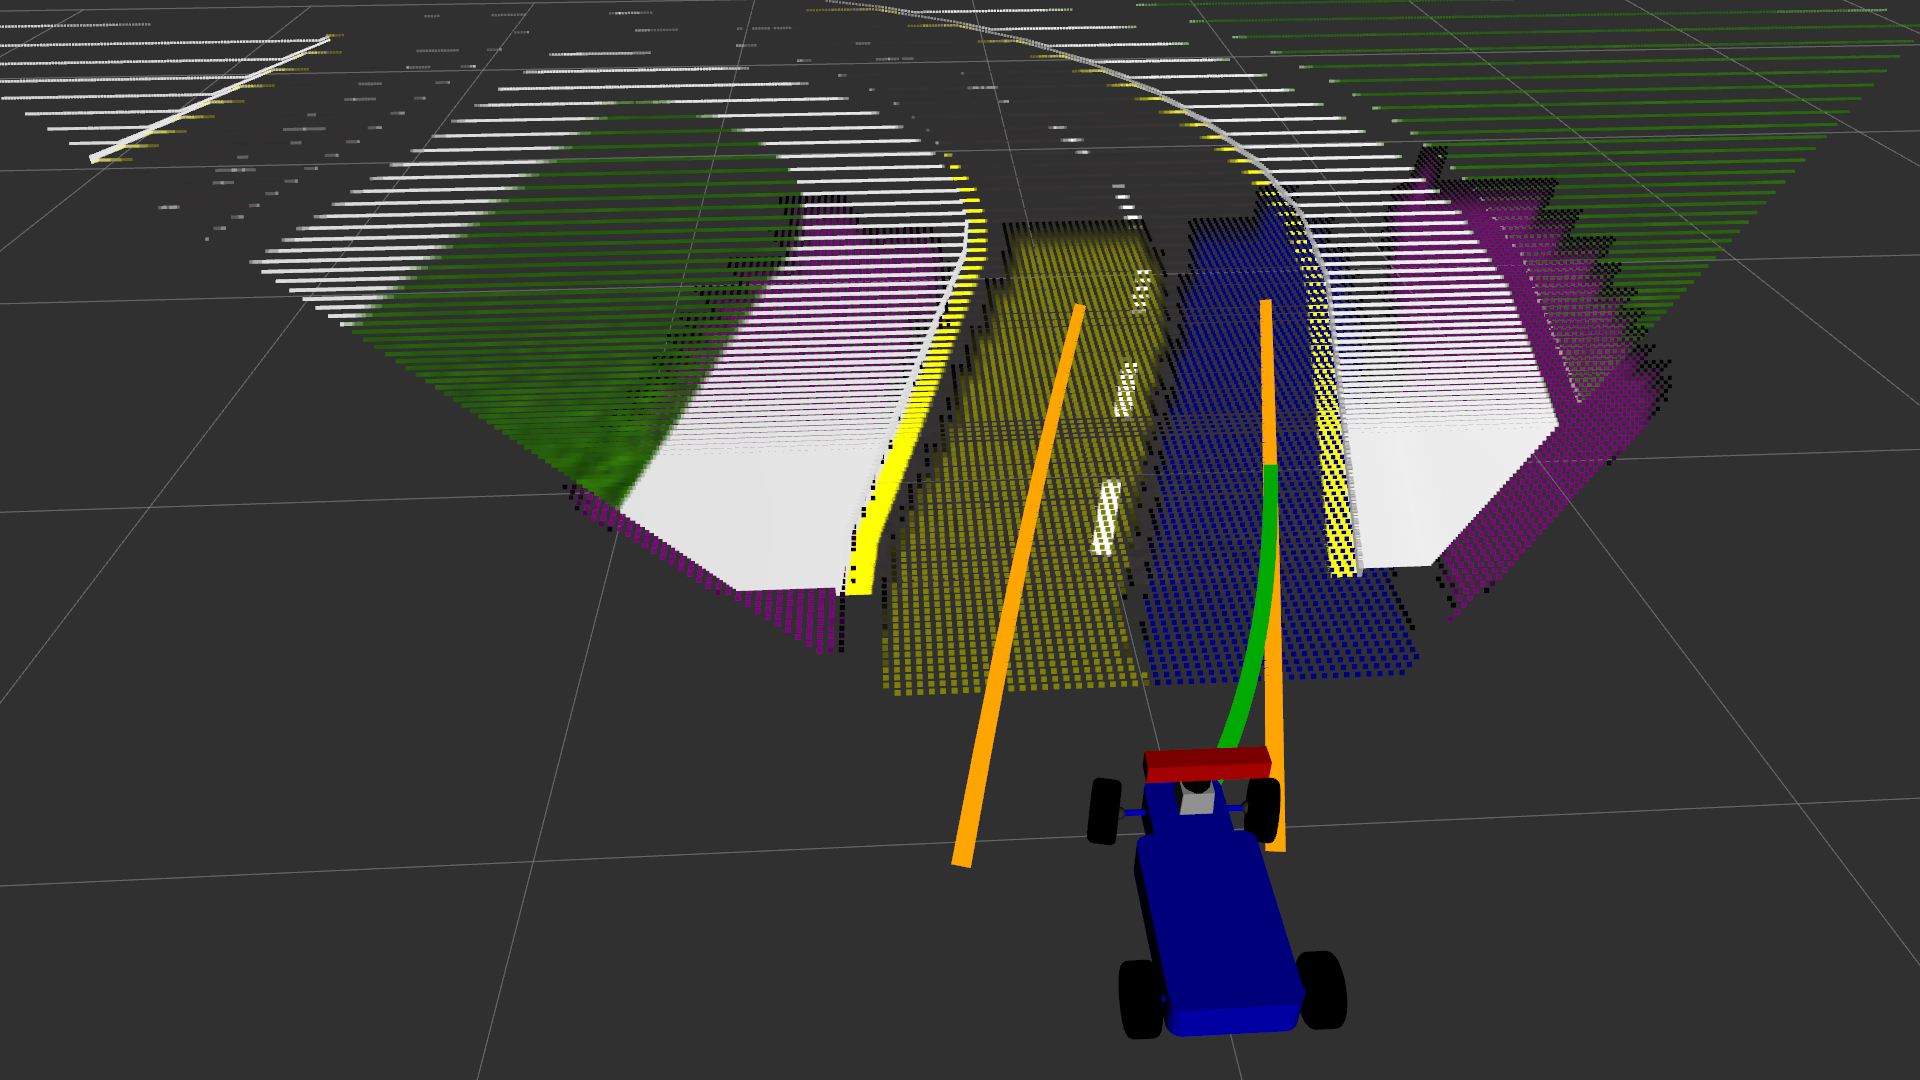
\includegraphics[width=\linewidth]{figures/experiments/overtaking4-pc.png}
  \end{subfigure}
  \caption{Experiments.}
  \label{figure:lane-change}
\end{figure}

\begin{figure}[h]
  \centering
  \begin{subfigure}[b]{0.45\linewidth}
      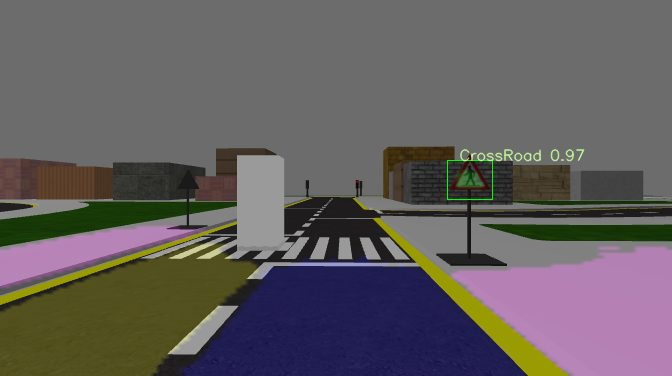
\includegraphics[width=\linewidth]{figures/experiments/cross-road-stop-img.png}
  \end{subfigure}
  \begin{subfigure}[b]{0.45\linewidth}
      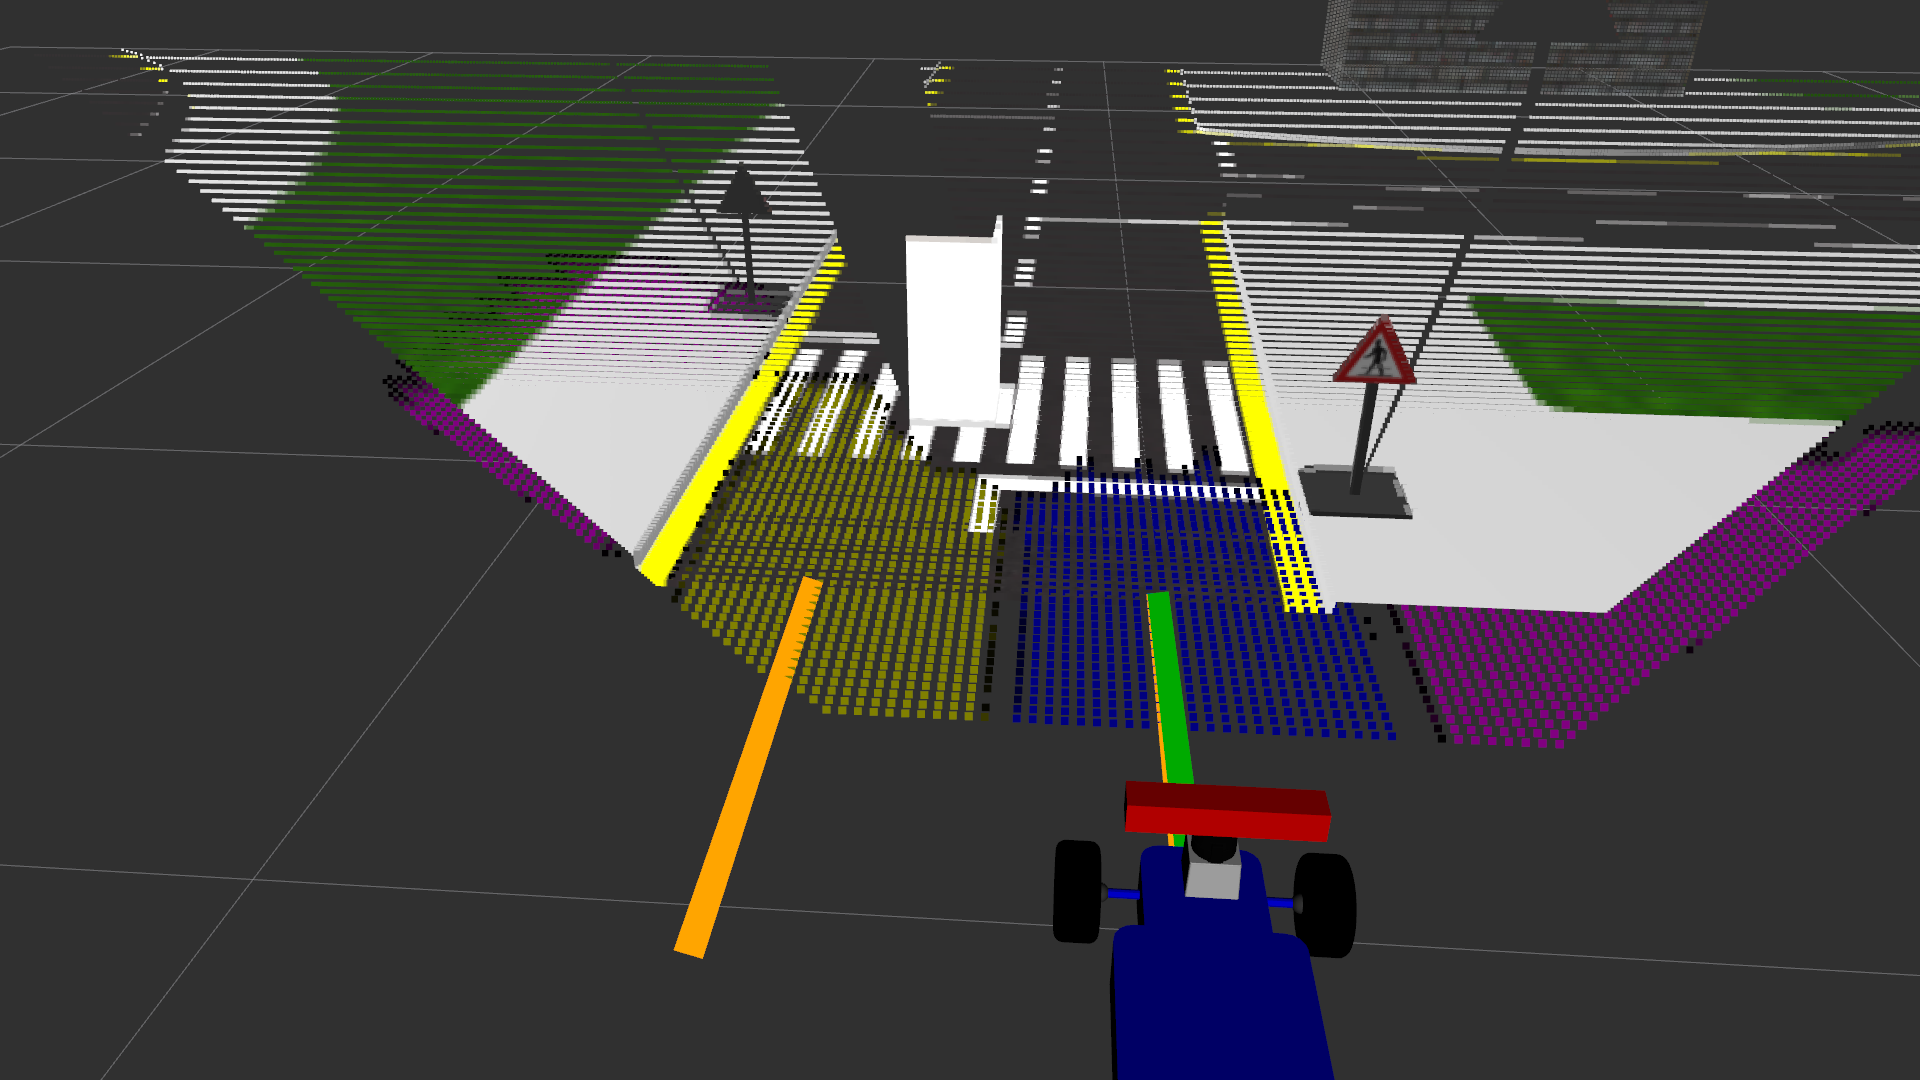
\includegraphics[width=\linewidth]{figures/experiments/cross-road-stop-pc.png}
  \end{subfigure}
  \begin{subfigure}[b]{0.45\linewidth}
      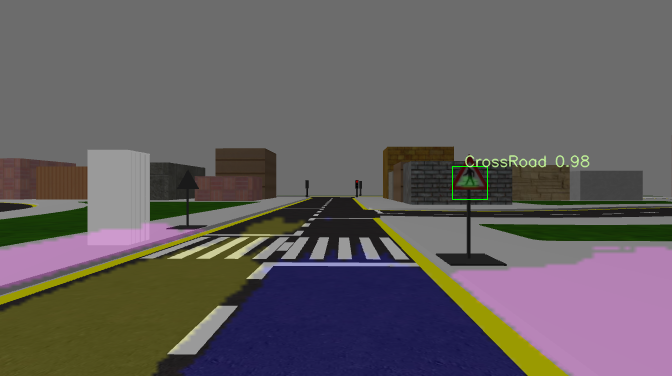
\includegraphics[width=\linewidth]{figures/experiments/cross-road-go-img.png}
  \end{subfigure}
  \begin{subfigure}[b]{0.45\linewidth}
      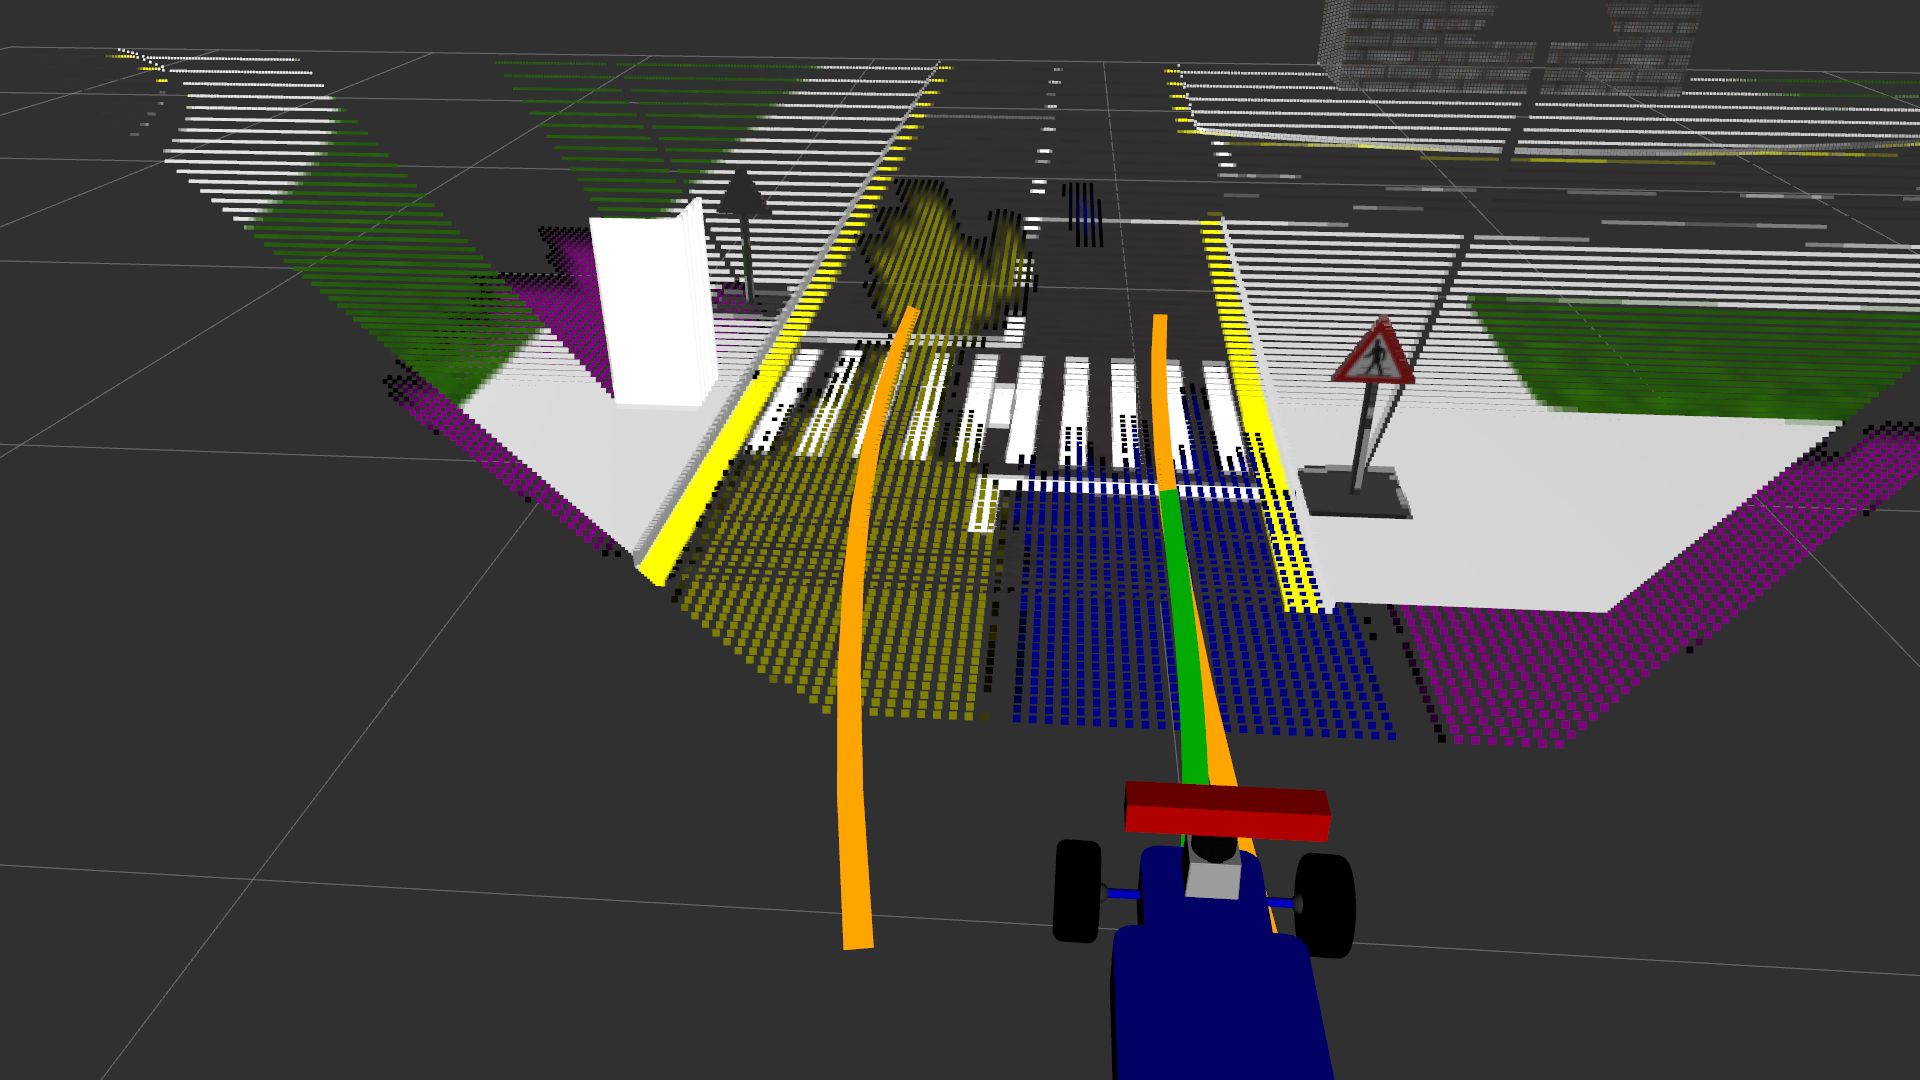
\includegraphics[width=\linewidth]{figures/experiments/cross-road-go-pc.png}
  \end{subfigure}
  \begin{subfigure}[b]{0.45\linewidth}
      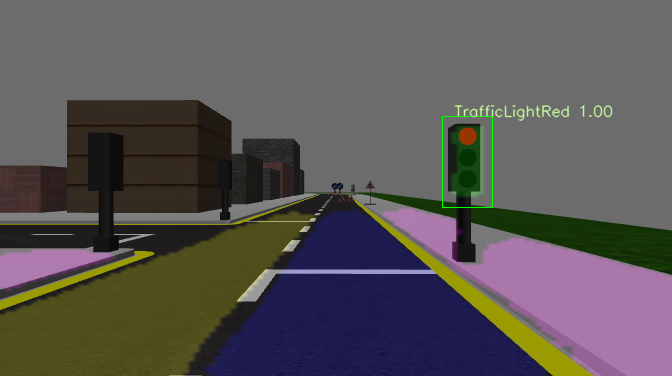
\includegraphics[width=\linewidth]{figures/experiments/red-light-stop-img.png}
  \end{subfigure}
  \begin{subfigure}[b]{0.45\linewidth}
      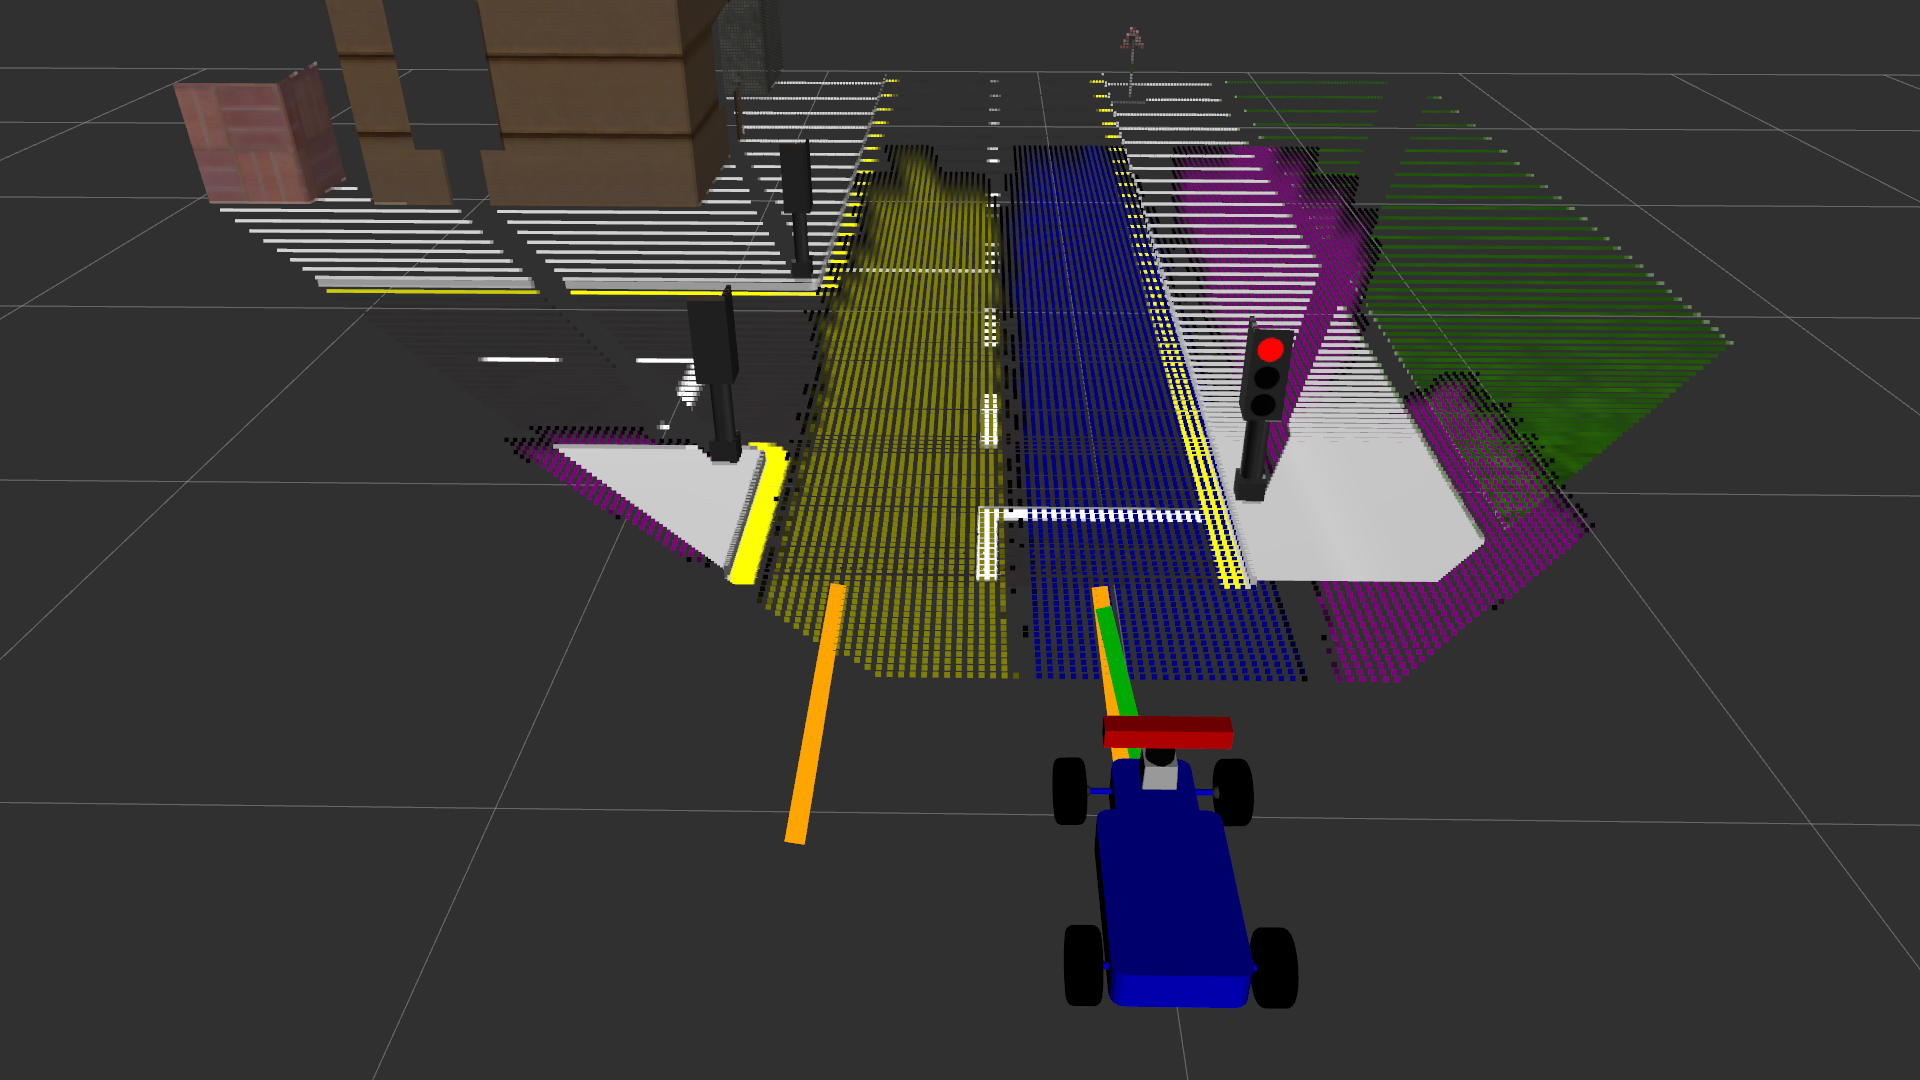
\includegraphics[width=\linewidth]{figures/experiments/red-light-stop-pc.png}
  \end{subfigure}
  \begin{subfigure}[b]{0.45\linewidth}
      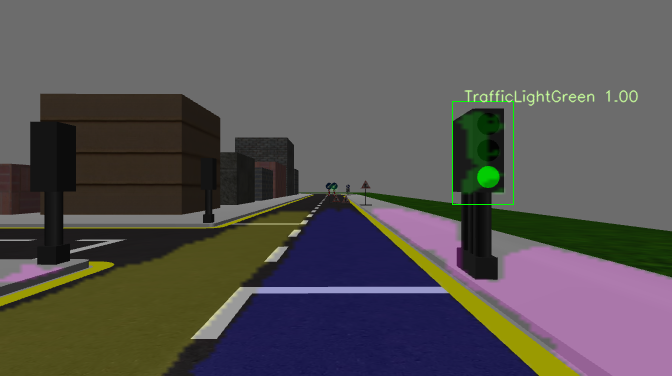
\includegraphics[width=\linewidth]{figures/experiments/green-light-go-img.png}
  \end{subfigure}
  \begin{subfigure}[b]{0.45\linewidth}
      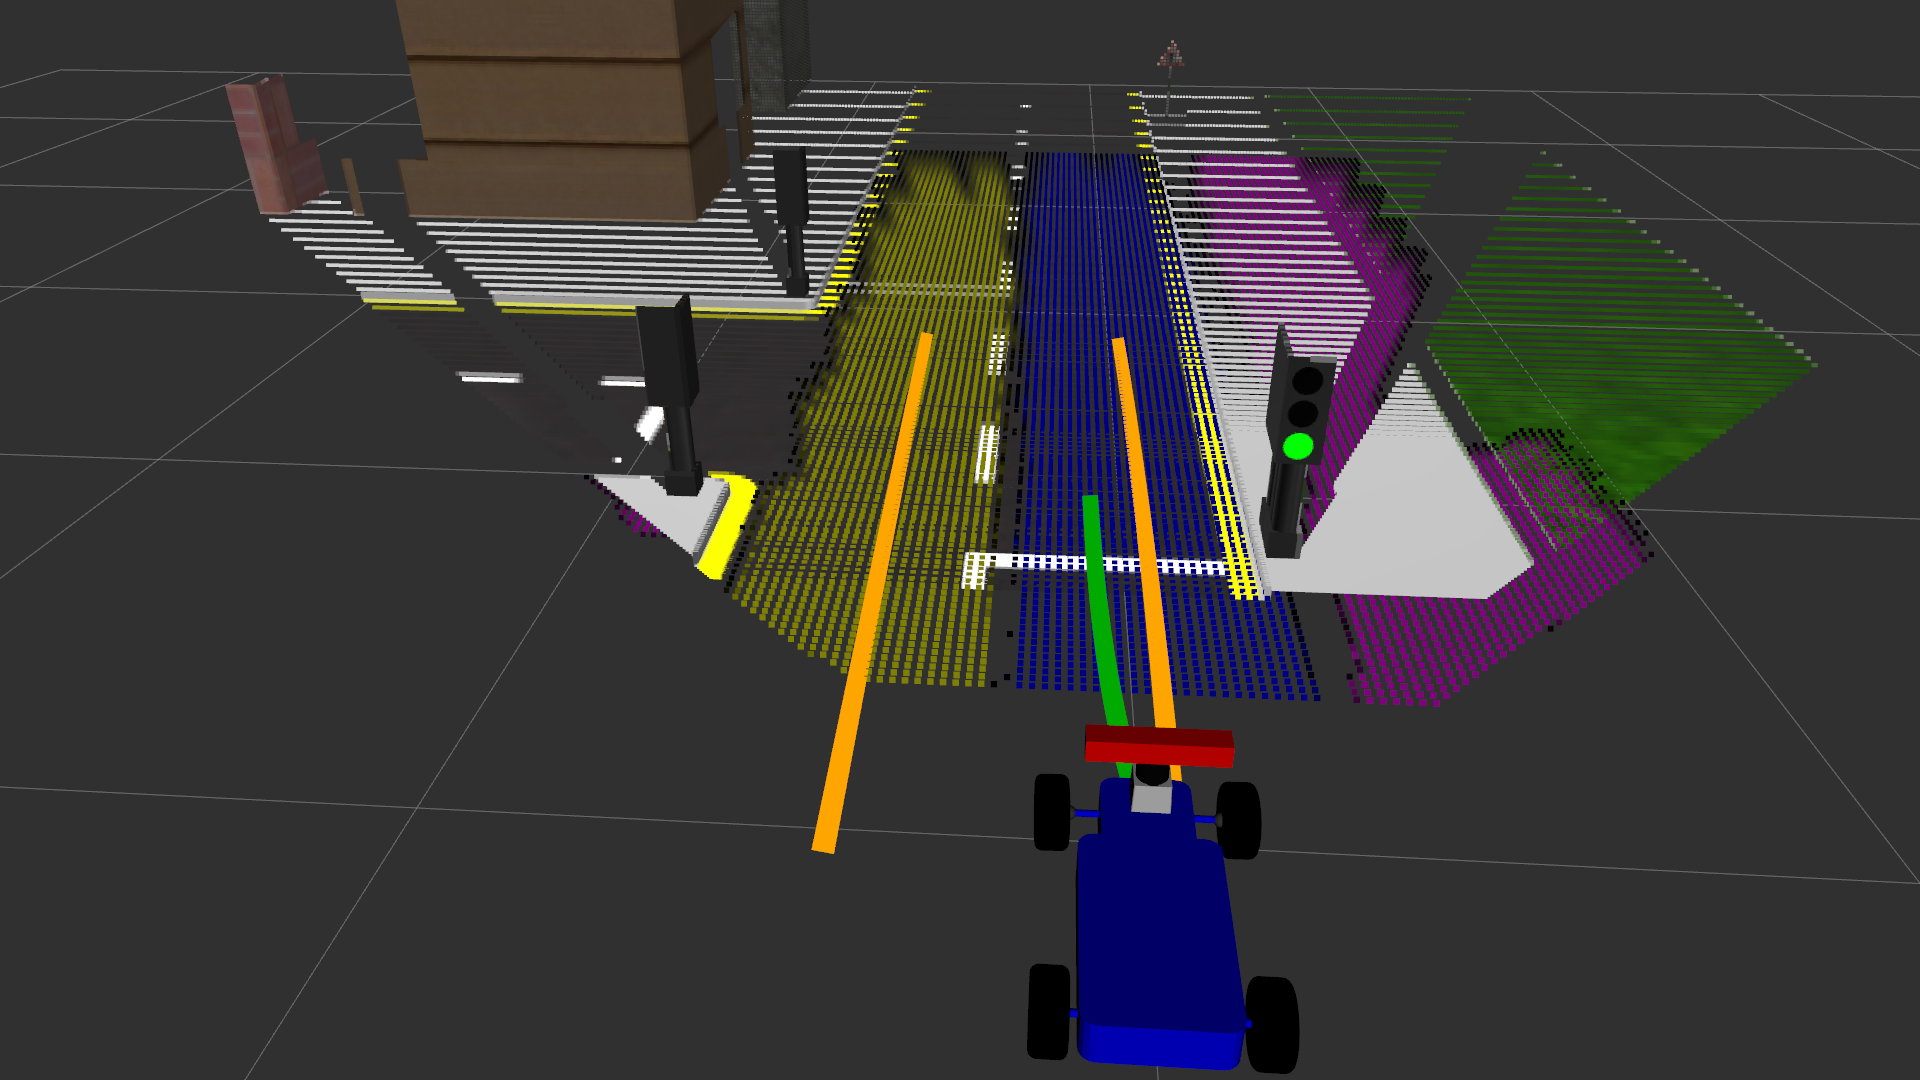
\includegraphics[width=\linewidth]{figures/experiments/green-light-go-pc.png}
  \end{subfigure}
  \begin{subfigure}[b]{0.45\linewidth}
      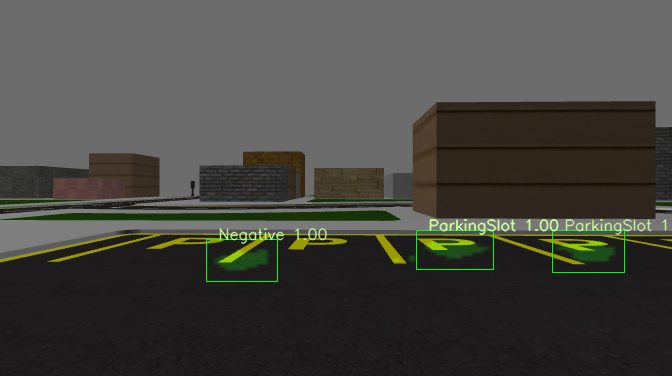
\includegraphics[width=\linewidth]{figures/experiments/parking-slot-img.png}
  \end{subfigure}
  \begin{subfigure}[b]{0.45\linewidth}
      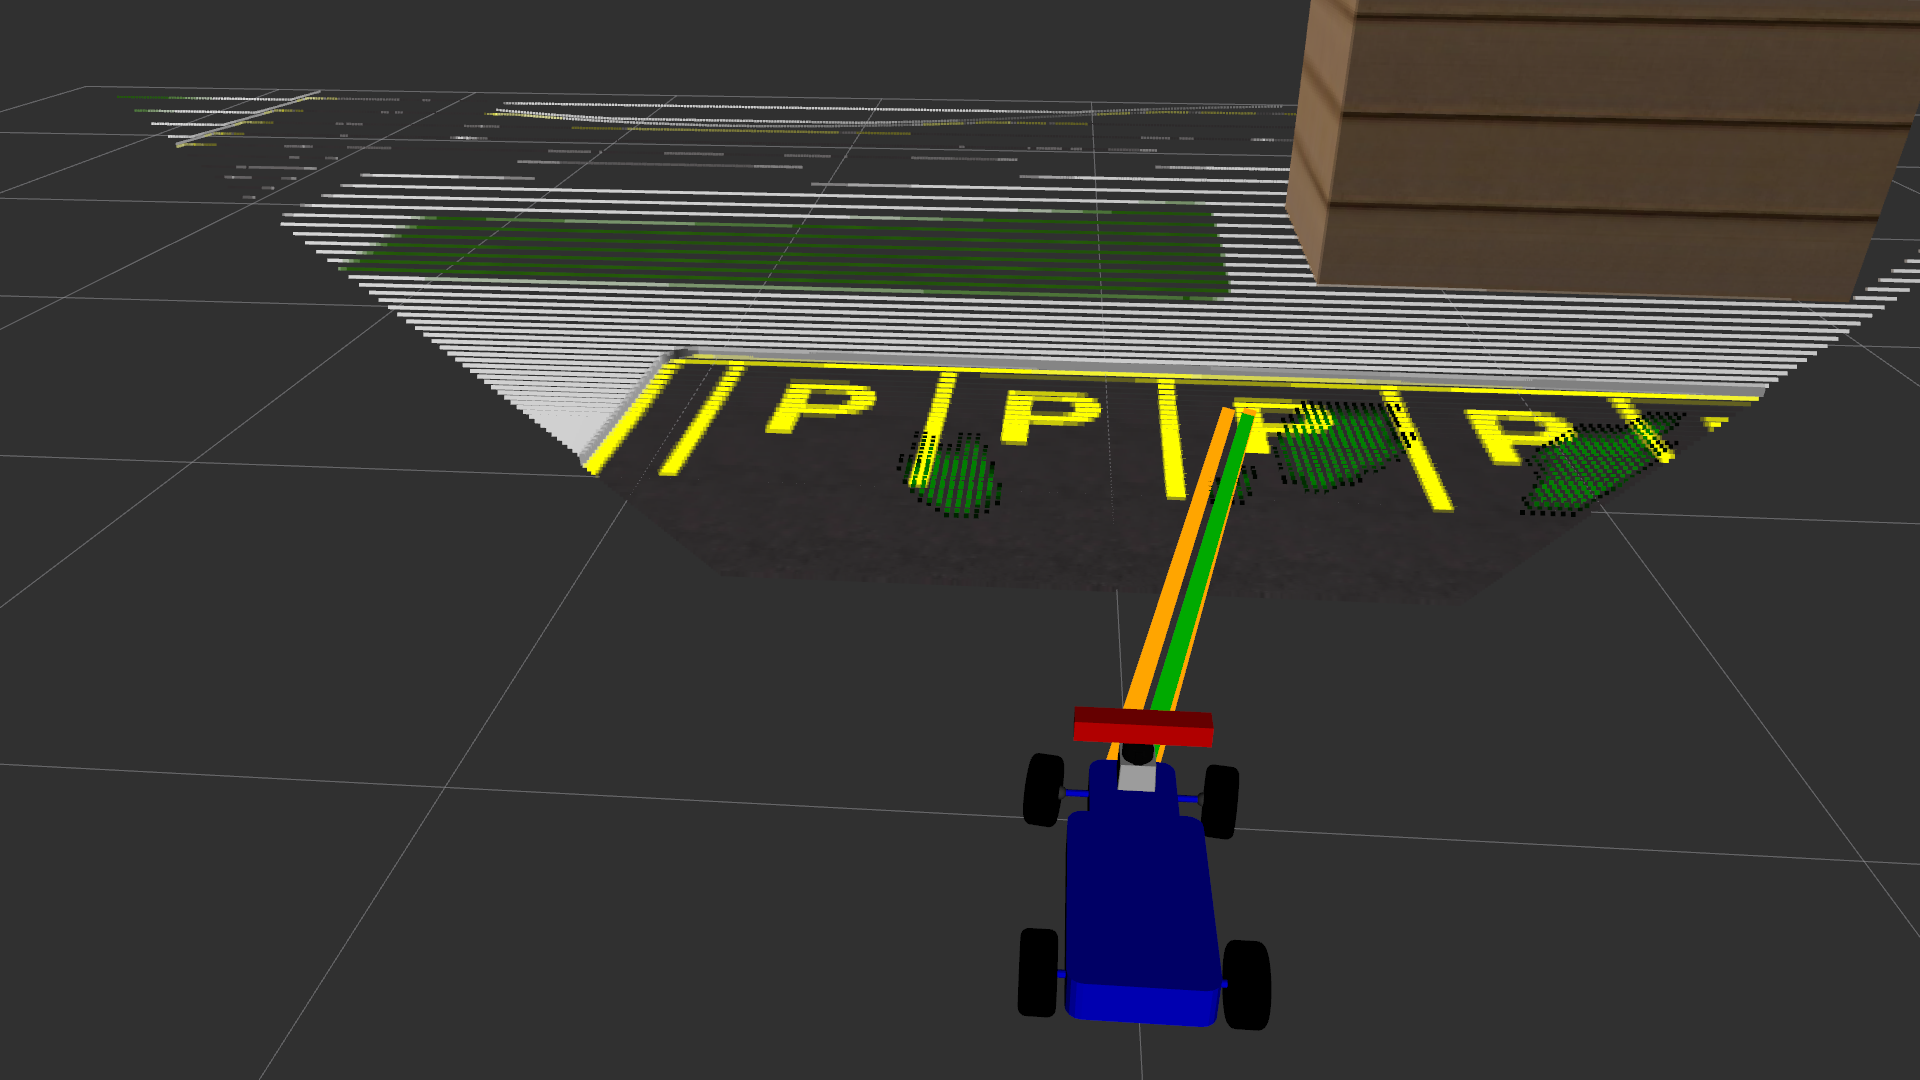
\includegraphics[width=\linewidth]{figures/experiments/parking-slot-pc.png}
  \end{subfigure}
  \caption{Experiments.}
  \label{figure:stop}
\end{figure}
